% $Header: /u/gcmpack/manual/s_examples/text/model_examples.tex,v 1.3 2002/12/17 14:39:53 mlosch Exp $
% $Name:  $

\section{Tutorials}
\label{sect:tutorials}
\label{www:tutorials}

This is the first in a series of tutorials describing
example MITgcm numerical experiments. The example experiments
include both straightforward examples of idealized geophysical
fluid simulations and more involved cases encompassing
large scale modeling and
automatic differentiation. Both hydrostatic and non-hydrostatic
experiments are presented, as well as experiments employing
Cartesian, spherical-polar and cube-sphere coordinate systems.
These ``case study'' documents include information describing
the experimental configuration and detailed information on how to
configure the MITgcm code and input files for each experiment.

\input{part3/case_studies/barotropic_gyre/baro.tex}

\newpage
% $Header: /u/gcmpack/manual/s_examples/baroclinic_gyre/fourlayer.tex,v 1.4 2001/10/24 19:43:07 cnh Exp $
% $Name:  $

\section{Example: Four layer Baroclinic Ocean Gyre In Spherical Coordinates}
\label{sec:eg-fourlayer}

\bodytext{bgcolor="#FFFFFFFF"}

%\begin{center} 
%{\Large \bf Using MITgcm to Simulate a Baroclinic Ocean Gyre In Spherical
%Polar Coordinates}
%
%\vspace*{4mm}
%
%\vspace*{3mm}
%{\large May 2001}
%\end{center}

This document describes an example experiment using MITgcm
to simulate a baroclinic ocean gyre in spherical
polar coordinates. The barotropic
example experiment in section \ref{sec:eg-baro}
ilustrated how to configure the code for a single layer 
simulation in a cartesian grid. In this example a similar physical problem
is simulated, but the code is now configured
for four layers and in a spherical polar coordinate system.

\subsection{Overview}

This example experiment demonstrates using the MITgcm to simulate
a baroclinic, wind-forced, ocean gyre circulation. The experiment 
is a numerical rendition of the gyre circulation problem simliar
to the problems described analytically by Stommel in 1966 
\cite{Stommel66} and numerically in Holland et. al \cite{Holland75}.
\\

In this experiment the model is configured to represent a mid-latitude 
enclosed sector of fluid on a sphere, $60^{\circ} \times 60^{\circ}$ in 
lateral extent. The fluid is $2$~km deep and is forced
by a constant in time zonal wind stress, $\tau_x$, that varies sinusoidally
in the north-south direction. Topologically the simulated 
domain is a sector on a sphere and the coriolis parameter, $f$, is defined 
according to latitude, $\varphi$

\begin{equation}
\label{EQ:fcori}
f(\varphi) = 2 \Omega \sin( \varphi )
\end{equation}
 
\noindent with the rotation rate, $\Omega$ set to $\frac{2 \pi}{86400s}$.
\\
  
 The sinusoidal wind-stress variations are defined according to 

\begin{equation}
\label{EQ:taux}
\tau_x(\varphi) = \tau_{0}\sin(\pi \frac{\varphi}{L_{\varphi}})
\end{equation}
 
\noindent where $L_{\varphi}$ is the lateral domain extent ($60^{\circ}$) and 
$\tau_0$ is set to $0.1N m^{-2}$. 
\\

Figure \ref{FIG:simulation_config}
summarises the configuration simulated.
In contrast to the example in section \ref{sec:eg-baro}, the 
current experiment simulates a spherical polar domain. However, as indicated
by the axes in the lower left of the figure the model code works internally
in a locally orthoganal coordinate $(x,y,z)$. For this experiment description 
of this document the local orthogonal model coordinate $(x,y,z)$ is synonomous 
with the spherical polar coordinate shown in figure 
\ref{fig:spherical-polar-coord}
\\

The experiment has four levels in the vertical, each of equal thickness,
$\Delta z = 500$~m. Initially the fluid is stratified with a reference
potential temperature profile,
$\theta_{250}=20^{\circ}$~C,
$\theta_{750}=10^{\circ}$~C,
$\theta_{1250}=8^{\circ}$~C,
$\theta_{1750}=6^{\circ}$~C. The equation of state used in this experiment is 
linear

\begin{equation}
\label{EQ:linear1_eos}
\rho = \rho_{0} ( 1 - \alpha_{\theta}\theta^{'} )
\end{equation}

\noindent which is implemented in the model as a density anomaly equation

\begin{equation}
\label{EQ:linear1_eos_pert}
\rho^{'} = -\rho_{0}\alpha_{\theta}\theta^{'}
\end{equation}

\noindent with $\rho_{0}=999.8\,{\rm kg\,m}^{-3}$ and 
$\alpha_{\theta}=2\times10^{-4}\,{\rm degrees}^{-1} $. Integrated forward in
this configuration the model state variable {\bf theta} is synonomous with
either in-situ temperature, $T$, or potential temperature, $\theta$. For 
consistency with later examples, in which the equation of state is
non-linear, we use $\theta$ to represent temperature here. This is
the quantity that is carried in the model core equations.

\begin{figure}
\begin{center}
 \resizebox{7.5in}{5.5in}{
   \includegraphics*[0.2in,0.7in][10.5in,10.5in]
   {part3/case_studies/fourlayer_gyre/simulation_config.eps} }
\end{center}
\caption{Schematic of simulation domain and wind-stress forcing function 
for the four-layer gyre numerical experiment. The domain is enclosed by solid
walls at $0^{\circ}$~E, $60^{\circ}$~E, $0^{\circ}$~N and $60^{\circ}$~N.
In the four-layer case an initial temperature stratification is 
imposed by setting the potential temperature, $\theta$, in each layer.
The vertical spacing, $\Delta z$, is constant and equal to $500$m.
}
\label{FIG:simulation_config}
\end{figure}

\subsection{Equations solved}

The implicit free surface form of the 
pressure equation described in Marshall et. al \cite{Marshall97a} is 
employed. 
A horizontal laplacian operator $\nabla_{h}^2$ provides viscous
dissipation. The wind-stress momentum input is added to the momentum equation
for the ``zonal flow'', $u$. Other terms in the model
are explicitly switched off for this experiement configuration (see section
\ref{SEC:code_config} ). This yields an active set of equations in 
solved in this configuration, written in spherical polar coordinates as 
follows

\begin{eqnarray}
\label{EQ:model_equations}
\frac{Du}{Dt} - fv + 
  \frac{1}{\rho}\frac{\partial p^{\prime}}{\partial \lambda} - 
  A_{h}\nabla_{h}^2u - A_{z}\frac{\partial^{2}u}{\partial z^{2}} 
& = &
\cal{F}
\\
\frac{Dv}{Dt} + fu + 
  \frac{1}{\rho}\frac{\partial p^{\prime}}{\partial \varphi} - 
  A_{h}\nabla_{h}^2v - A_{z}\frac{\partial^{2}v}{\partial z^{2}} 
& = &
0
\\
\frac{\partial \eta}{\partial t} + \frac{\partial H \hat{u}}{\partial \lambda} +
\frac{\partial H \hat{v}}{\partial \varphi}
&=&
0
\\
\frac{D\theta}{Dt} -
 K_{h}\nabla_{h}^2\theta  - K_{z}\frac{\partial^{2}\theta}{\partial z^{2}} 
& = &
0
\\
p^{\prime} & = &
g\rho_{0} \eta + \int^{0}_{-z}\rho^{\prime} dz
\\
\rho^{\prime} & = &- \alpha_{\theta}\rho_{0}\theta^{\prime}
\\
{\cal F} |_{s} & = & \frac{\tau_{x}}{\rho_{0}\Delta z_{s}}
\\
{\cal F} |_{i} & = & 0
\end{eqnarray}

\noindent where $u$ and $v$ are the components of the horizontal
flow vector $\vec{u}$ on the sphere ($u=\dot{\lambda},v=\dot{\varphi}$).
The terms $H\hat{u}$ and $H\hat{v}$ are the components of the term
integrated in eqaution \ref{eq:free-surface}, as descirbed in section

The suffices ${s},{i}$ indicate surface and interior of the domain.
The forcing $\cal F$ is only applied at the surface.
The pressure field, $p^{\prime}$, is separated into a barotropic part
due to variations in sea-surface height, $\eta$, and a hydrostatic
part due to variations in density, $\rho^{\prime}$, over the water column.

\subsection{Discrete Numerical Configuration}

 The model is configured in hydrostatic form.  The domain is discretised with 
a uniform grid spacing in latitude and longitude
 $\Delta \lambda=\Delta \varphi=1^{\circ}$, so 
that there are sixty grid cells in the zonal and meridional directions. 
Vertically the 
model is configured with four layers with constant depth, 
$\Delta z$, of $500$~m. The internal, locally orthogonal, model coordinate 
variables $x$ and $y$ are initialised from the values of
$\lambda$, $\varphi$, $\Delta \lambda$ and $\Delta \varphi$ in
radians according to

\begin{eqnarray}
x=r\cos(\varphi)\lambda,~\Delta x & = &r\cos(\varphi)\Delta \lambda \\
y=r\varphi,~\Delta y &= &r\Delta \varphi
\end{eqnarray}

The procedure for generating a set of internal grid variables from a
spherical polar grid specification is discussed in section 
\ref{sec:spatial_discrete_horizontal_grid}.

\noindent\fbox{ \begin{minipage}{5.5in}
{\em S/R INI\_SPHERICAL\_POLAR\_GRID} ({\em
model/src/ini\_spherical\_polar\_grid.F})

$A_c$, $A_\zeta$, $A_w$, $A_s$: {\bf rAc}, {\bf rAz}, {\bf rAw}, {\bf rAs}
({\em GRID.h})

$\Delta x_g$, $\Delta y_g$: {\bf DXg}, {\bf DYg} ({\em GRID.h})

$\Delta x_c$, $\Delta y_c$: {\bf DXc}, {\bf DYc} ({\em GRID.h})

$\Delta x_f$, $\Delta y_f$: {\bf DXf}, {\bf DYf} ({\em GRID.h})

$\Delta x_v$, $\Delta y_u$: {\bf DXv}, {\bf DYu} ({\em GRID.h})

\end{minipage} }\\



As described in \ref{sec:tracer_equations}, the time evolution of potential 
temperature, 
$\theta$, equation is solved prognostically.
The pressure forces that drive the fluid motions, (
$\frac{\partial p^{'}}{\partial \lambda}$ and $\frac{\partial p^{'}}{\partial \varphi}$), are found by summing pressure due to surface 
elevation $\eta$ and the hydrostatic pressure.

\subsubsection{Numerical Stability Criteria}

The laplacian dissipation coefficient, $A_{h}$, is set to $400 m s^{-1}$.
This value is chosen to yield a Munk layer width \cite{Adcroft_thesis},

\begin{eqnarray}
\label{EQ:munk_layer}
M_{w} = \pi ( \frac { A_{h} }{ \beta } )^{\frac{1}{3}}
\end{eqnarray}

\noindent  of $\approx 100$km. This is greater than the model
resolution in mid-latitudes $\Delta x$, ensuring that the frictional 
boundary layer is well resolved.
\\

\noindent The model is stepped forward with a 
time step $\delta t=1200$secs. With this time step the stability 
parameter to the horizontal laplacian friction \cite{Adcroft_thesis}

\begin{eqnarray}
\label{EQ:laplacian_stability}
S_{l} = 4 \frac{A_{h} \delta t}{{\Delta x}^2}
\end{eqnarray}

\noindent evaluates to 0.012, which is well below the 0.3 upper limit
for stability. 
\\

\noindent The vertical dissipation coefficient, $A_{z}$, is set to 
$1\times10^{-2} {\rm m}^2{\rm s}^{-1}$. The associated stability limit

\begin{eqnarray}
\label{EQ:laplacian_stability_z}
S_{l} = 4 \frac{A_{z} \delta t}{{\Delta z}^2}
\end{eqnarray}

\noindent evaluates to $4.8 \times 10^{-5}$ which is again well below
the upper limit.
The values of $A_{h}$ and $A_{z}$ are also used for the horizontal ($K_{h}$) 
and vertical ($K_{z}$) diffusion coefficients for temperature respectively.
\\

\noindent The numerical stability for inertial oscillations
\cite{Adcroft_thesis} 

\begin{eqnarray}
\label{EQ:inertial_stability}
S_{i} = f^{2} {\delta t}^2
\end{eqnarray}

\noindent evaluates to $0.0144$, which is well below the $0.5$ upper 
limit for stability.
\\

\noindent The advective CFL \cite{Adcroft_thesis} for a extreme maximum 
horizontal flow
speed of $ | \vec{u} | = 2 ms^{-1}$

\begin{eqnarray}
\label{EQ:cfl_stability}
S_{a} = \frac{| \vec{u} | \delta t}{ \Delta x}
\end{eqnarray}

\noindent evaluates to $5 \times 10^{-2}$. This is well below the stability 
limit of 0.5.
\\

\noindent The stability parameter for internal gravity waves 
\cite{Adcroft_thesis}

\begin{eqnarray}
\label{EQ:igw_stability}
S_{c} = \frac{c_{g} \delta t}{ \Delta x}
\end{eqnarray}

\noindent evaluates to $5 \times 10^{-2}$. This is well below the linear
stability limit of 0.25.
  
\subsection{Code Configuration}
\label{SEC:code_config}

The model configuration for this experiment resides under the 
directory {\it verification/exp1/}.  The experiment files 
\begin{itemize}
\item {\it input/data}
\item {\it input/data.pkg}
\item {\it input/eedata},
\item {\it input/windx.sin\_y},
\item {\it input/topog.box},
\item {\it code/CPP\_EEOPTIONS.h}
\item {\it code/CPP\_OPTIONS.h},
\item {\it code/SIZE.h}. 
\end{itemize}
contain the code customisations and parameter settings for this 
experiements. Below we describe the customisations
to these files associated with this experiment.

\subsubsection{File {\it input/data}}

This file, reproduced completely below, specifies the main parameters 
for the experiment. The parameters that are significant for this configuration
are

\begin{itemize}

\item Line 4, 
\begin{verbatim} tRef=20.,10.,8.,6., \end{verbatim} 
this line sets
the initial and reference values of potential temperature at each model
level in units of $^{\circ}$C.
The entries are ordered from surface to depth. For each
depth level the inital and reference profiles will be uniform in
$x$ and $y$. The values specified here are read into the
variable 
{\bf
\begin{rawhtml} <A href=../../../code_reference/vdb/names/OK.htm> \end{rawhtml}
tRef
\begin{rawhtml} </A>\end{rawhtml}
} 
in the model code, by procedure 
{\it
\begin{rawhtml} <A href=../../../code_reference/vdb/code/94.htm> \end{rawhtml}
INI\_PARMS
\begin{rawhtml} </A>\end{rawhtml}
}.

%% \codelink{var:tref} tRef \endlink
%% \codelink{file:ini_parms} {\it INI\_PARMS } \endlink
%% \codelink{proc:ini_parms} {\it INI\_PARMS } \endlink
%% \var{tref}
%% \proc{ini_parms}
%% \file{ini_parms}
\newcommand{\VARtref}{
{\bf
\begin{rawhtml} <A href=../../../code_reference/vdb/names/OK.htm> \end{rawhtml}
tRef
\begin{rawhtml} </A>\end{rawhtml}
} 
}



\fbox{
\begin{minipage}{5.0in}
{\it S/R INI\_THETA}
({\it ini\_theta.F})
\end{minipage}
}
{\bf
\begin{rawhtml} <A href=../../../code_reference/vdb/code/98.htm> \end{rawhtml}
goto code
\begin{rawhtml} </A>\end{rawhtml}
}


\item Line 6, 
\begin{verbatim} viscAz=1.E-2, \end{verbatim} 
this line sets the vertical laplacian dissipation coefficient to
$1 \times 10^{-2} {\rm m^{2}s^{-1}}$. Boundary conditions
for this operator are specified later. 
The variable 
{\bf 
\begin{rawhtml} <A href=../../../code_reference/vdb/names/ZQ.htm> \end{rawhtml}
viscAz
\begin{rawhtml} </A>\end{rawhtml}
}
is read in the routine
{\it
\begin{rawhtml} <A href=../../../code_reference/vdb/code/94.htm> \end{rawhtml}
INI\_PARMS
\begin{rawhtml} </A>\end{rawhtml}
}
and is copied into model general vertical coordinate variable 
{\bf 
\begin{rawhtml} <A href=../../../code_reference/vdb/names/PF.htm> \end{rawhtml}
viscAr
\begin{rawhtml} </A>\end{rawhtml}
}.

\fbox{
\begin{minipage}{5.0in}
{\it S/R CALC\_DIFFUSIVITY}({\it calc\_diffusivity.F})
\end{minipage}
}
{\bf
\begin{rawhtml} <A href=../../../code_reference/vdb/code/53.htm> \end{rawhtml}
goto code
\begin{rawhtml} </A>\end{rawhtml}
}

\item Line 7, 
\begin{verbatim}
viscAh=4.E2,
\end{verbatim} 
this line sets the horizontal laplacian frictional dissipation coefficient to
$1 \times 10^{-2} {\rm m^{2}s^{-1}}$. Boundary conditions
for this operator are specified later.
The variable 
{\bf 
\begin{rawhtml} <A href=../../../code_reference/vdb/names/SI.htm> \end{rawhtml}
viscAh
\begin{rawhtml} </A>\end{rawhtml}
}
is read in the routine
{\it
\begin{rawhtml} <A href=../../../code_reference/vdb/code/94.htm> \end{rawhtml}
INI\_PARMS
\begin{rawhtml} </A>\end{rawhtml}
}.

\fbox{
\begin{minipage}{5.0in}
{\it S/R CALC\_MOM\_RHS}({\it calc\_mom\_rhs.F})
\end{minipage}
}
{\bf
\begin{rawhtml} <A href=../../../code_reference/vdb/code/60.htm> \end{rawhtml}
goto code
\begin{rawhtml} </A>\end{rawhtml}
}

\fbox{
\begin{minipage}{5.0in}
{\it S/R CALC\_GW}({\it calc\_gw.F})
\end{minipage}
}
{\bf
\begin{rawhtml} <A href=../../../code_reference/vdb/code/58.htm> \end{rawhtml}
goto code
\begin{rawhtml} </A>\end{rawhtml}
}

\item Lines 8,
\begin{verbatim}
no_slip_sides=.FALSE.
\end{verbatim}
this line selects a free-slip lateral boundary condition for
the horizontal laplacian friction operator 
e.g. $\frac{\partial u}{\partial y}$=0 along boundaries in $y$ and
$\frac{\partial v}{\partial x}$=0 along boundaries in $x$.
The variable
{\bf
\begin{rawhtml} <A href=../../../code_reference/vdb/names/UT.htm> \end{rawhtml}
no\_slip\_sides
\begin{rawhtml} </A>\end{rawhtml}
}
is read in the routine
{\it
\begin{rawhtml} <A href=../../../code_reference/vdb/code/94.htm> \end{rawhtml}
INI\_PARMS
\begin{rawhtml} </A>\end{rawhtml}
}.


\fbox{
\begin{minipage}{5.0in}
{\it S/R CALC\_MOM\_RHS}({\it calc\_mom\_rhs.F})
\end{minipage}
}
{\bf
\begin{rawhtml} <A href=../../../code_reference/vdb/code/60.htm> \end{rawhtml}
goto code
\begin{rawhtml} </A>\end{rawhtml}
}

\item Lines 9,
\begin{verbatim}
no_slip_bottom=.TRUE.
\end{verbatim}
this line selects a no-slip boundary condition for bottom
boundary condition in the vertical laplacian friction operator 
e.g. $u=v=0$ at $z=-H$, where $H$ is the local depth of the domain.
The variable
{\bf
\begin{rawhtml} <A href=../../../code_reference/vdb/names/UK.htm> \end{rawhtml}
no\_slip\_bottom
\begin{rawhtml} </A>\end{rawhtml}
}
is read in the routine
{\it
\begin{rawhtml} <A href=../../../code_reference/vdb/code/94.htm> \end{rawhtml}
INI\_PARMS
\begin{rawhtml} </A>\end{rawhtml}
}.

\fbox{
\begin{minipage}{5.0in}
{\it S/R CALC\_MOM\_RHS}({\it calc\_mom\_rhs.F})
\end{minipage}
}
{\bf
\begin{rawhtml} <A href=../../../code_reference/vdb/code/60.htm> \end{rawhtml}
goto code
\begin{rawhtml} </A>\end{rawhtml}
}

\item Line 10,
\begin{verbatim}
diffKhT=4.E2,
\end{verbatim}
this line sets the horizontal diffusion coefficient for temperature
to $400\,{\rm m^{2}s^{-1}}$. The boundary condition on this
operator is $\frac{\partial}{\partial x}=\frac{\partial}{\partial y}=0$ at
all boundaries.
The variable
{\bf
\begin{rawhtml} <A href=../../../code_reference/vdb/names/RC.htm> \end{rawhtml}
diffKhT
\begin{rawhtml} </A>\end{rawhtml}
}
is read in the routine
{\it
\begin{rawhtml} <A href=../../../code_reference/vdb/code/94.htm> \end{rawhtml}
INI\_PARMS
\begin{rawhtml} </A>\end{rawhtml}
}.

\fbox{ \begin{minipage}{5.0in}
{\it S/R CALC\_GT}({\it calc\_gt.F})
\end{minipage}
}
{\bf
\begin{rawhtml} <A href=../../../code_reference/vdb/code/57.htm> \end{rawhtml}
goto code
\begin{rawhtml} </A>\end{rawhtml}
}

\item Line 11,
\begin{verbatim}
diffKzT=1.E-2,
\end{verbatim}
this line sets the vertical diffusion coefficient for temperature
to $10^{-2}\,{\rm m^{2}s^{-1}}$. The boundary condition on this
operator is $\frac{\partial}{\partial z}$ = 0 on all boundaries.
The variable
{\bf
\begin{rawhtml} <A href=../../../code_reference/vdb/names/ZT.htm> \end{rawhtml}
diffKzT
\begin{rawhtml} </A>\end{rawhtml}
}
is read in the routine
{\it
\begin{rawhtml} <A href=../../../code_reference/vdb/code/94.htm> \end{rawhtml}
INI\_PARMS
\begin{rawhtml} </A>\end{rawhtml}
}.
It is copied into model general vertical coordinate variable
{\bf
\begin{rawhtml} <A href=../../../code_reference/vdb/names/PD.htm> \end{rawhtml}
diffKrT
\begin{rawhtml} </A>\end{rawhtml}
}.

\fbox{ \begin{minipage}{5.0in}
{\it S/R CALC\_DIFFUSIVITY}({\it calc\_diffusivity.F})
\end{minipage}
}
{\bf
\begin{rawhtml} <A href=../../../code_reference/vdb/code/53.htm> \end{rawhtml}
goto code
\begin{rawhtml} </A>\end{rawhtml}
}



\item Line 13,
\begin{verbatim}
tAlpha=2.E-4,
\end{verbatim}
This line sets the thermal expansion coefficient for the fluid
to $2 \times 10^{-4}\,{\rm degrees}^{-1}$
The variable
{\bf
\begin{rawhtml} <A href=../../../code_reference/vdb/names/ZV.htm> \end{rawhtml}
tAlpha 
\begin{rawhtml} </A>\end{rawhtml}
}
is read in the routine
{\it
\begin{rawhtml} <A href=../../../code_reference/vdb/code/94.htm> \end{rawhtml}
INI\_PARMS
\begin{rawhtml} </A>\end{rawhtml}
}.

\fbox{
\begin{minipage}{5.0in}
{\it S/R FIND\_RHO}({\it find\_rho.F})
\end{minipage}
}
{\bf
\begin{rawhtml} <A href=../../../code_reference/vdb/code/79.htm> \end{rawhtml}
goto code
\begin{rawhtml} </A>\end{rawhtml}
}

\item Line 18,
\begin{verbatim}
eosType='LINEAR'
\end{verbatim}
This line selects the linear form of the equation of state.
The variable
{\bf
\begin{rawhtml} <A href=../../../code_reference/vdb/names/WV.htm> \end{rawhtml}
eosType
\begin{rawhtml} </A>\end{rawhtml}
}
is read in the routine
{\it
\begin{rawhtml} <A href=../../../code_reference/vdb/code/94.htm> \end{rawhtml}
INI\_PARMS
\begin{rawhtml} </A>\end{rawhtml}
}.

\fbox{
\begin{minipage}{5.0in}
{\it S/R FIND\_RHO}({\it find\_rho.F})
\end{minipage}
}
{\bf
\begin{rawhtml} <A href=../../../code_reference/vdb/code/79.htm> \end{rawhtml}
goto code
\begin{rawhtml} </A>\end{rawhtml}
}



\item Line 40,
\begin{verbatim}
usingSphericalPolarGrid=.TRUE.,
\end{verbatim}
This line requests that the simulation be performed in a 
spherical polar coordinate system. It affects the interpretation of
grid inoput parameters, for exampl {\bf delX} and {\bf delY} and
causes the grid generation routines to initialise an internal grid based
on spherical polar geometry.
The variable
{\bf
\begin{rawhtml} <A href=../../../code_reference/vdb/names/10T.htm> \end{rawhtml}
usingSphericalPolarGrid
\begin{rawhtml} </A>\end{rawhtml}
}
is read in the routine
{\it
\begin{rawhtml} <A href=../../../code_reference/vdb/code/94.htm> \end{rawhtml}
INI\_PARMS
\begin{rawhtml} </A>\end{rawhtml}
}.

\fbox{
\begin{minipage}{5.0in}
{\it S/R INI\_SPEHRICAL\_POLAR\_GRID}({\it ini\_spherical\_polar\_grid.F})
\end{minipage}
}
{\bf
\begin{rawhtml} <A href=../../../code_reference/vdb/code/97.htm> \end{rawhtml}
goto code
\begin{rawhtml} </A>\end{rawhtml}
}

\item Line 41,
\begin{verbatim}
phiMin=0.,
\end{verbatim}
This line sets the southern boundary of the modeled
domain to $0^{\circ}$ latitude. This value affects both the
generation of the locally orthogonal grid that the model
uses internally and affects the initialisation of the coriolis force.
Note - it is not required to set
a longitude boundary, since the absolute longitude does
not alter the kernel equation discretisation.
The variable
{\bf
\begin{rawhtml} <A href=../../../code_reference/vdb/names/110.htm> \end{rawhtml}
phiMin
\begin{rawhtml} </A>\end{rawhtml}
}
is read in the routine
{\it
\begin{rawhtml} <A href=../../../code_reference/vdb/code/94.htm> \end{rawhtml}
INI\_PARMS
\begin{rawhtml} </A>\end{rawhtml}
}.

\fbox{
\begin{minipage}{5.0in}
{\it S/R INI\_SPEHRICAL\_POLAR\_GRID}({\it ini\_spherical\_polar\_grid.F})
\end{minipage}
}
{\bf
\begin{rawhtml} <A href=../../../code_reference/vdb/code/97.htm> \end{rawhtml}
goto code
\begin{rawhtml} </A>\end{rawhtml}
}

\item Line 42,
\begin{verbatim}
delX=60*1.,
\end{verbatim}
This line sets the horizontal grid spacing between each y-coordinate line
in the discrete grid to $1^{\circ}$ in longitude.
The variable
{\bf
\begin{rawhtml} <A href=../../../code_reference/vdb/names/10Z.htm> \end{rawhtml}
delX
\begin{rawhtml} </A>\end{rawhtml}
}
is read in the routine
{\it
\begin{rawhtml} <A href=../../../code_reference/vdb/code/94.htm> \end{rawhtml}
INI\_PARMS
\begin{rawhtml} </A>\end{rawhtml}
}.

\fbox{
\begin{minipage}{5.0in}
{\it S/R INI\_SPEHRICAL\_POLAR\_GRID}({\it ini\_spherical\_polar\_grid.F})
\end{minipage}
}
{\bf
\begin{rawhtml} <A href=../../../code_reference/vdb/code/97.htm> \end{rawhtml}
goto code
\begin{rawhtml} </A>\end{rawhtml}
}

\item Line 43,
\begin{verbatim}
delY=60*1.,
\end{verbatim}
This line sets the horizontal grid spacing between each y-coordinate line
in the discrete grid to $1^{\circ}$ in latitude.
The variable
{\bf
\begin{rawhtml} <A href=../../../code_reference/vdb/names/UB.htm> \end{rawhtml}
delY   
\begin{rawhtml} </A>\end{rawhtml}
}
is read in the routine
{\it
\begin{rawhtml} <A href=../../../code_reference/vdb/code/94.htm> \end{rawhtml}
INI\_PARMS
\begin{rawhtml} </A>\end{rawhtml}
}.

\fbox{
\begin{minipage}{5.0in}
{\it S/R INI\_SPEHRICAL\_POLAR\_GRID}({\it ini\_spherical\_polar\_grid.F})
\end{minipage}
}
{\bf
\begin{rawhtml} <A href=../../../code_reference/vdb/code/97.htm> \end{rawhtml}
goto code
\begin{rawhtml} </A>\end{rawhtml}
}

\item Line 44,
\begin{verbatim}
delZ=500.,500.,500.,500.,
\end{verbatim}
This line sets the vertical grid spacing between each z-coordinate line
in the discrete grid to $500\,{\rm m}$, so that the total model depth 
is $2\,{\rm km}$.
The variable
{\bf
\begin{rawhtml} <A href=../../../code_reference/vdb/names/10W.htm> \end{rawhtml}
delZ
\begin{rawhtml} </A>\end{rawhtml}
}
is read in the routine
{\it
\begin{rawhtml} <A href=../../../code_reference/vdb/code/94.htm> \end{rawhtml}
INI\_PARMS
\begin{rawhtml} </A>\end{rawhtml}
}.
It is copied into the internal
model coordinate variable 
{\bf 
\begin{rawhtml} <A href=../../../code_reference/vdb/names/10Y.htm> \end{rawhtml}
delR
\begin{rawhtml} </A>\end{rawhtml}
}. 

\fbox{
\begin{minipage}{5.0in}
{\it S/R INI\_VERTICAL\_GRID}({\it ini\_vertical\_grid.F})
\end{minipage}
}
{\bf
\begin{rawhtml} <A href=../../../code_reference/vdb/code/100.htm> \end{rawhtml}
goto code
\begin{rawhtml} </A>\end{rawhtml}
}

\item Line 47,
\begin{verbatim}
bathyFile='topog.box'
\end{verbatim}
This line specifies the name of the file from which the domain
bathymetry is read. This file is a two-dimensional ($x,y$) map of
depths. This file is assumed to contain 64-bit binary numbers 
giving the depth of the model at each grid cell, ordered with the x 
coordinate varying fastest. The points are ordered from low coordinate
to high coordinate for both axes. The units and orientation of the
depths in this file are the same as used in the MITgcm code. In this
experiment, a depth of $0m$ indicates a solid wall and a depth
of $-2000m$ indicates open ocean. The matlab program
{\it input/gendata.m} shows an example of how to generate a
bathymetry file.
The variable
{\bf
\begin{rawhtml} <A href=../../../code_reference/vdb/names/179.htm> \end{rawhtml}
bathyFile
\begin{rawhtml} </A>\end{rawhtml}
}
is read in the routine
{\it
\begin{rawhtml} <A href=../../../code_reference/vdb/code/94.htm> \end{rawhtml}
INI\_PARMS
\begin{rawhtml} </A>\end{rawhtml}
}.

\fbox{
\begin{minipage}{5.0in}
{\it S/R INI\_DEPTHS}({\it ini\_depths.F})
\end{minipage}
}
{\bf
\begin{rawhtml} <A href=../../../code_reference/vdb/code/88.htm> \end{rawhtml}
goto code
\begin{rawhtml} </A>\end{rawhtml}
}


\item Line 50,
\begin{verbatim}
zonalWindFile='windx.sin_y'
\end{verbatim}
This line specifies the name of the file from which the x-direction
surface wind stress is read. This file is also a two-dimensional
($x,y$) map and is enumerated and formatted in the same manner as the 
bathymetry file. The matlab program {\it input/gendata.m} includes example 
code to generate a valid 
{\bf zonalWindFile} 
file.  
The variable
{\bf
\begin{rawhtml} <A href=../../../code_reference/vdb/names/13W.htm> \end{rawhtml}
zonalWindFile
\begin{rawhtml} </A>\end{rawhtml}
}
is read in the routine
{\it
\begin{rawhtml} <A href=../../../code_reference/vdb/code/94.htm> \end{rawhtml}
INI\_PARMS
\begin{rawhtml} </A>\end{rawhtml}
}.

\fbox{
\begin{minipage}{5.0in}
{\it S/R EXTERNAL\_FIELDS\_LOAD}({\it external\_fields\_load.F})
\end{minipage}
}
{\bf
\begin{rawhtml} <A href=../../../code_reference/vdb/code/75.htm> \end{rawhtml}
goto code
\begin{rawhtml} </A>\end{rawhtml}
}

\end{itemize}

\noindent other lines in the file {\it input/data} are standard values
that are described in the MITgcm Getting Started and MITgcm Parameters
notes.

\begin{rawhtml}<PRE>\end{rawhtml}
\begin{small}
% $Header: /u/gcmpack/manual/s_examples/baroclinic_gyre/input/data.tex,v 1.1.1.1 2001/08/08 16:15:46 adcroft Exp $
% $Name:  $

\begin{verbatim}
     1	# Model parameters
     2	# Continuous equation parameters
     3	 &PARM01
     4	 tRef=20.,10.,8.,6.,
     5	 sRef=10.,10.,10.,10.,
     6	 viscAz=1.E-2,
     7	 viscAh=4.E2,
     8	 no_slip_sides=.FALSE.,
     9	 no_slip_bottom=.TRUE.,
    10	 diffKhT=4.E2,
    11	 diffKzT=1.E-2,
    12	 beta=1.E-11,
    13	 tAlpha=2.E-4,
    14	 sBeta =0.,
    15	 gravity=9.81,
    16	 rigidLid=.FALSE.,
    17	 implicitFreeSurface=.TRUE.,
    18	 eosType='LINEAR',
    19	 readBinaryPrec=64,
    20	 &
    21	# Elliptic solver parameters
    22	 &PARM02
    23	 cg2dMaxIters=1000,
    24	 cg2dTargetResidual=1.E-13,
    25	 &
    26	# Time stepping parameters
    27	 &PARM03
    28	 startTime=0.,
    29	 endTime=12000., 
    30	 deltaTmom=1200.0,
    31	 deltaTtracer=1200.0,
    32	 abEps=0.1,
    33	 pChkptFreq=17000.0,
    34	 chkptFreq=0.0,
    35	 dumpFreq=2592000.0,
    36	 &
    37	# Gridding parameters
    38	 &PARM04
    39	 usingCartesianGrid=.FALSE.,
    40	 usingSphericalPolarGrid=.TRUE.,
    41	 phiMin=0.,
    42	 delX=60*1.,
    43	 delY=60*1.,
    44	 delZ=500.,500.,500.,500.,
    45	 &
    46	 &PARM05
    47	 bathyFile='topog.box',
    48	 hydrogThetaFile=,
    49	 hydrogSaltFile=,
    50	 zonalWindFile='windx.sin_y',
    51	 meridWindFile=,
    52	 &
\end{verbatim}

\end{small}
\begin{rawhtml}</PRE>\end{rawhtml}

\subsubsection{File {\it input/data.pkg}}

This file uses standard default values and does not contain
customisations for this experiment.

\subsubsection{File {\it input/eedata}}

This file uses standard default values and does not contain
customisations for this experiment.

\subsubsection{File {\it input/windx.sin\_y}}

The {\it input/windx.sin\_y} file specifies a two-dimensional ($x,y$) 
map of wind stress ,$\tau_{x}$, values. The units used are $Nm^{-2}$.
Although $\tau_{x}$ is only a function of $y$n in this experiment
this file must still define a complete two-dimensional map in order
to be compatible with the standard code for loading forcing fields 
in MITgcm. The included matlab program {\it input/gendata.m} gives a complete
code for creating the {\it input/windx.sin\_y} file.

\subsubsection{File {\it input/topog.box}}


The {\it input/topog.box} file specifies a two-dimensional ($x,y$) 
map of depth values. For this experiment values are either
$0m$ or $-2000\,{\rm m}$, corresponding respectively to a wall or to deep
ocean. The file contains a raw binary stream of data that is enumerated
in the same way as standard MITgcm two-dimensional, horizontal arrays.
The included matlab program {\it input/gendata.m} gives a complete
code for creating the {\it input/topog.box} file.

\subsubsection{File {\it code/SIZE.h}}

Two lines are customized in this file for the current experiment

\begin{itemize}

\item Line 39, 
\begin{verbatim} sNx=60, \end{verbatim} this line sets
the lateral domain extent in grid points for the
axis aligned with the x-coordinate.

\item Line 40, 
\begin{verbatim} sNy=60, \end{verbatim} this line sets
the lateral domain extent in grid points for the
axis aligned with the y-coordinate.

\item Line 49, 
\begin{verbatim} Nr=4,   \end{verbatim} this line sets
the vertical domain extent in grid points.

\end{itemize}

\begin{small}
% $Header: /u/gcmpack/manual/s_examples/barotropic_gyre/code/SIZE.h.tex,v 1.1.1.1 2001/08/08 16:15:58 adcroft Exp $
% $Name:  $

\begin{verbatim}
     1	C $Header: /u/gcmpack/manual/s_examples/barotropic_gyre/code/SIZE.h.tex,v 1.1.1.1 2001/08/08 16:15:58 adcroft Exp $
     2	C $Name:  $
     3	C
     4	C     /==========================================================\
     5	C     | SIZE.h Declare size of underlying computational grid.    |
     6	C     |==========================================================|
     7	C     | The design here support a three-dimensional model grid   |
     8	C     | with indices I,J and K. The three-dimensional domain     |
     9	C     | is comprised of nPx*nSx blocks of size sNx along one axis|
    10	C     | nPy*nSy blocks of size sNy along another axis and one    |
    11	C     | block of size Nz along the final axis.                   |
    12	C     | Blocks have overlap regions of size OLx and OLy along the|
    13	C     | dimensions that are subdivided.                          |
    14	C     \==========================================================/
    15	C     Voodoo numbers controlling data layout.
    16	C     sNx - No. X points in sub-grid.
    17	C     sNy - No. Y points in sub-grid.
    18	C     OLx - Overlap extent in X.
    19	C     OLy - Overlat extent in Y.
    20	C     nSx - No. sub-grids in X.
    21	C     nSy - No. sub-grids in Y.
    22	C     nPx - No. of processes to use in X.
    23	C     nPy - No. of processes to use in Y.
    24	C     Nx  - No. points in X for the total domain.
    25	C     Ny  - No. points in Y for the total domain.
    26	C     Nr  - No. points in R for full process domain.
    27	      INTEGER sNx
    28	      INTEGER sNy
    29	      INTEGER OLx
    30	      INTEGER OLy
    31	      INTEGER nSx
    32	      INTEGER nSy
    33	      INTEGER nPx
    34	      INTEGER nPy
    35	      INTEGER Nx
    36	      INTEGER Ny
    37	      INTEGER Nr
    38	      PARAMETER (
    39	     &           sNx =  60,
    40	     &           sNy =  60,
    41	     &           OLx =   3,
    42	     &           OLy =   3,
    43	     &           nSx =   1,
    44	     &           nSy =   1,
    45	     &           nPx =   1,
    46	     &           nPy =   1,
    47	     &           Nx  = sNx*nSx*nPx,
    48	     &           Ny  = sNy*nSy*nPy,
    49	     &           Nr  =   1)
       
    50	C     MAX_OLX  - Set to the maximum overlap region size of any array
    51	C     MAX_OLY    that will be exchanged. Controls the sizing of exch
    52	C                routine buufers.
    53	      INTEGER MAX_OLX
    54	      INTEGER MAX_OLY
    55	      PARAMETER ( MAX_OLX = OLx,
    56	     &            MAX_OLY = OLy )
\end{verbatim}

\end{small}

\subsubsection{File {\it code/CPP\_OPTIONS.h}}

This file uses standard default values and does not contain
customisations for this experiment.


\subsubsection{File {\it code/CPP\_EEOPTIONS.h}}

This file uses standard default values and does not contain
customisations for this experiment.

\subsubsection{Other Files }

Other files relevant to this experiment are
\begin{itemize}
\item {\it model/src/ini\_cori.F}. This file initializes the model
coriolis variables {\bf fCorU} and {\bf fCorV}.
\item {\it model/src/ini\_spherical\_polar\_grid.F} This file
initializes the model grid discretisation variables {\bf
dxF, dyF, dxG, dyG, dxC, dyC}.
\item {\it model/src/ini\_parms.F}.
\end{itemize}

\subsection{Running The Example}
\label{SEC:running_the_example}

\subsubsection{Code Download}

 In order to run the examples you must first download the code distribution.
Instructions for downloading the code can be found in the Getting Started
Guide \cite{MITgcm_Getting_Started}.

\subsubsection{Experiment Location}

 This example experiments is located under the release sub-directory

\vspace{5mm}
{\it verification/exp1/ }

\subsubsection{Running the Experiment}

 To run the experiment

\begin{enumerate}
\item Set the current directory to {\it input/ }

\begin{verbatim}
% cd input
\end{verbatim}

\item Verify that current directory is now correct

\begin{verbatim}
% pwd
\end{verbatim}

 You shold see a response on the screen ending in

{\it verification/exp1/input }


\item Run the genmake script to create the experiment {\it Makefile}

\begin{verbatim}
% ../../../tools/genmake -mods=../code
\end{verbatim}

\item Create a list of header file dependencies in {\it Makefile}

\begin{verbatim}
% make depend
\end{verbatim}

\item Build the executable file.

\begin{verbatim}
% make
\end{verbatim}

\item Run the {\it mitgcmuv} executable

\begin{verbatim}
% ./mitgcmuv
\end{verbatim}

\end{enumerate}




\newpage
% $Header: /u/gcmpack/manual/s_examples/global_oce_latlon/climatalogical_ogcm.tex,v 1.2 2001/10/22 11:55:48 cnh Exp $
% $Name:  $

\section{Example: 4$^\circ$ Global Climatological Ocean Simulation}
\label{sec:eg-global}

\bodytext{bgcolor="#FFFFFFFF"}

%\begin{center} 
%{\Large \bf Using MITgcm to Simulate Global Climatalogical Ocean Circulation
%At Four Degree Resolution with Asynchronous Time Stepping}
%
%\vspace*{4mm}
%
%\vspace*{3mm}
%{\large May 2001}
%\end{center}

\subsection{Introduction}

This document describes the third example MITgcm experiment. The first
two examples illustrated how to configure the code for hydrostatic idealised
geophysical fluids simulations. This example iilustrates the use of
the MITgcm for large scale ocean circulation simulation.

\subsection{Overview}

This example experiment demonstrates using the MITgcm to simulate
the planetary ocean circulation. The simulation is configured
with realistic geography and bathymetry on a
$4^{\circ} \times 4^{\circ}$ spherical polar grid.
Twenty levels are used in the vertical, ranging in thickness
from $50\,{\rm m}$ at the surface to $815\,{\rm m}$ at depth,
giving a maximum model depth of $6\,{\rm km}$.
At this resolution, the configuration
can be integrated forward for thousands of years on a single 
processor desktop computer.
\\

The model is forced with climatalogical wind stress data and surface
flux data from DaSilva \cite{DaSilva94}. Climatalogical data
from Levitus \cite{Levitus94} is used to initialise the model hydrography.
Levitus seasonal clmatology data is also used throughout the calculation
to provide additional air-sea fluxes.
These fluxes are combined with the DaSilva climatalogical estimates of
surface heat flux and fresh water, resulting in a mixed boundary
condition of the style decribed in Haney \cite{Haney}.
Altogether, this yields the following forcing applied
in the model surface layer.

\begin{eqnarray}
\label{EQ:global_forcing}
\label{EQ:global_forcing_fu}
{\cal F}_{u} & = & \frac{\tau_{x}}{\rho_{0} \Delta z_{s}}
\\
\label{EQ:global_forcing_fv}
{\cal F}_{v} & = & \frac{\tau_{y}}{\rho_{0} \Delta z_{s}}
\\
\label{EQ:global_forcing_ft}
{\cal F}_{\theta} & = & - \lambda_{\theta} ( \theta - \theta^{\ast} ) 
 - \frac{1}{C_{p} \rho_{0} \Delta z_{s}}{\cal Q}
\\
\label{EQ:global_forcing_fs}
{\cal F}_{s} & = & - \lambda_{s} ( S - S^{\ast} ) 
 + \frac{S_{0}}{\Delta z_{s}}({\cal E} - {\cal P} - {\cal R})
\end{eqnarray}

\noindent where ${\cal F}_{u}$, ${\cal F}_{v}$, ${\cal F}_{\theta}$,
${\cal F}_{s}$ are the forcing terms in the zonal and meridional
momentum and in the potential temperature and salinity
equations respectively.
The term $\Delta z_{s}$ represents the top ocean layer thickness in
meters.
It is used in conjunction with a reference density, $\rho_{0}$
(here set to $999.8\,{\rm kg\,m^{-3}}$), a
reference salinity, $S_{0}$ (here set to 35~ppt),
and a specific heat capacity, $C_{p}$ (here set to
$4000~{\rm J}~^{\circ}{\rm C}^{-1}~{\rm kg}^{-1}$), to convert
input dataset values into time tendencies of
potential temperature (with units of $^{\circ}{\rm C}~{\rm s}^{-1}$),
salinity (with units ${\rm ppt}~s^{-1}$) and
velocity (with units ${\rm m}~{\rm s}^{-2}$).
The externally supplied forcing fields used in this
experiment are $\tau_{x}$, $\tau_{y}$, $\theta^{\ast}$, $S^{\ast}$,
$\cal{Q}$ and $\cal{E}-\cal{P}-\cal{R}$. The wind stress fields ($\tau_x$, $\tau_y$)
have units of ${\rm N}~{\rm m}^{-2}$. The temperature forcing fields
($\theta^{\ast}$ and $Q$) have units of $^{\circ}{\rm C}$ and ${\rm W}~{\rm m}^{-2}$
respectively. The salinity forcing fields ($S^{\ast}$ and 
$\cal{E}-\cal{P}-\cal{R}$) have units of ${\rm ppt}$ and ${\rm m}~{\rm s}^{-1}$
respectively.
\\


Figures (\ref{FIG:sim_config_tclim}-\ref{FIG:sim_config_empmr}) show the
relaxation temperature ($\theta^{\ast}$) and salinity ($S^{\ast}$) fields,
the wind stress components ($\tau_x$ and $\tau_y$), the heat flux ($Q$)
and the net fresh water flux (${\cal E} - {\cal P} - {\cal R}$) used
in equations \ref{EQ:global_forcing_fu}-\ref{EQ:global_forcing_fs}. The figures
also indicate the lateral extent and coastline used in the experiment.
Figure ({\ref{FIG:model_bathymetry}) shows the depth contours of the model
domain.


\subsection{Discrete Numerical Configuration}


 The model is configured in hydrostatic form.  The domain is discretised with 
a uniform grid spacing in latitude and longitude on the sphere
 $\Delta \phi=\Delta \lambda=4^{\circ}$, so 
that there are ninety grid cells in the zonal and forty in the 
meridional direction. The internal model coordinate variables
$x$ and $y$ are initialised according to
\begin{eqnarray}
x=r\cos(\phi),~\Delta x & = &r\cos(\Delta \phi) \\
y=r\lambda,~\Delta x &= &r\Delta \lambda 
\end{eqnarray}

Arctic polar regions are not
included in this experiment. Meridionally the model extends from
$80^{\circ}{\rm S}$ to $80^{\circ}{\rm N}$.
Vertically the model is configured with twenty layers with the 
following thicknesses
$\Delta z_{1} = 50\,{\rm m},\,
 \Delta z_{2} = 50\,{\rm m},\,
 \Delta z_{3} = 55\,{\rm m},\,
 \Delta z_{4} = 60\,{\rm m},\,
 \Delta z_{5} = 65\,{\rm m},\,
$
$
 \Delta z_{6}~=~70\,{\rm m},\,
 \Delta z_{7}~=~80\,{\rm m},\,
 \Delta z_{8}~=95\,{\rm m},\,
 \Delta z_{9}=120\,{\rm m},\,
 \Delta z_{10}=155\,{\rm m},\,
$
$
 \Delta z_{11}=200\,{\rm m},\,
 \Delta z_{12}=260\,{\rm m},\,
 \Delta z_{13}=320\,{\rm m},\,
 \Delta z_{14}=400\,{\rm m},\,
 \Delta z_{15}=480\,{\rm m},\,
$
$
 \Delta z_{16}=570\,{\rm m},\,
 \Delta z_{17}=655\,{\rm m},\,
 \Delta z_{18}=725\,{\rm m},\,
 \Delta z_{19}=775\,{\rm m},\,
 \Delta z_{20}=815\,{\rm m}
$ (here the numeric subscript indicates the model level index number, ${\tt k}$).
The implicit free surface form of the pressure equation described in Marshall et. al 
\cite{Marshall97a} is employed. A laplacian operator, $\nabla^2$, provides viscous
dissipation. Thermal and haline diffusion is also represented by a laplacian operator.

Wind-stress forcing is added to the momentum equations for both
the zonal flow, $u$ and the merdional flow $v$, according to equations 
(\ref{EQ:global_forcing_fu}) and (\ref{EQ:global_forcing_fv}).
Thermodynamic forcing inputs are added to the equations for
potential temperature, $\theta$, and salinity, $S$, according to equations 
(\ref{EQ:global_forcing_ft}) and (\ref{EQ:global_forcing_fs}).
This produces a set of equations solved in this configuration as follows:

\begin{eqnarray}
\label{EQ:model_equations}
\frac{Du}{Dt} - fv + 
  \frac{1}{\rho}\frac{\partial p^{'}}{\partial x} - 
  \nabla_{h}\cdot A_{h}\nabla_{h}u - 
  \frac{\partial}{\partial z}A_{z}\frac{\partial u}{\partial z} 
 & = &
\begin{cases}
{\cal F}_u & \text{(surface)} \\
0 & \text{(interior)}
\end{cases}
\\
\frac{Dv}{Dt} + fu + 
  \frac{1}{\rho}\frac{\partial p^{'}}{\partial y} - 
  \nabla_{h}\cdot A_{h}\nabla_{h}v - 
  \frac{\partial}{\partial z}A_{z}\frac{\partial v}{\partial z} 
& = &
\begin{cases}
{\cal F}_v & \text{(surface)} \\
0 & \text{(interior)}
\end{cases}
\\
\frac{\partial \eta}{\partial t} + \nabla_{h}\cdot \vec{u}
&=&
0
\\
\frac{D\theta}{Dt} -
 \nabla_{h}\cdot K_{h}\nabla_{h}\theta
 - \frac{\partial}{\partial z}\Gamma(K_{z})\frac{\partial\theta}{\partial z} 
& = &
\begin{cases}
{\cal F}_\theta & \text{(surface)} \\
0 & \text{(interior)}
\end{cases}
\\
\frac{D s}{Dt} -
 \nabla_{h}\cdot K_{h}\nabla_{h}s
 - \frac{\partial}{\partial z}\Gamma(K_{z})\frac{\partial s}{\partial z} 
& = &
\begin{cases}
{\cal F}_s & \text{(surface)} \\
0 & \text{(interior)}
\end{cases}
\\
g\rho_{0} \eta + \int^{0}_{-z}\rho^{'} dz & = & p^{'}
\end{eqnarray}

\noindent where $u=\frac{Dx}{Dt}=r \cos(\phi)\frac{D \lambda}{Dt}$ and 
$v=\frac{Dy}{Dt}=r \frac{D \phi}{Dt}$ 
are the zonal and meridional components of the
flow vector, $\vec{u}$, on the sphere. As described in
MITgcm Numerical Solution Procedure \cite{MITgcm_Numerical_Scheme}, the time 
evolution of potential temperature, $\theta$, equation is solved prognostically.
The total pressure, $p$, is diagnosed by summing pressure due to surface 
elevation $\eta$ and the hydrostatic pressure.
\\

\subsubsection{Numerical Stability Criteria}

The laplacian dissipation coefficient, $A_{h}$, is set to $5 \times 10^5 m s^{-1}$.
This value is chosen to yield a Munk layer width \cite{Adcroft_thesis},
\begin{eqnarray}
\label{EQ:munk_layer}
M_{w} = \pi ( \frac { A_{h} }{ \beta } )^{\frac{1}{3}}
\end{eqnarray}

\noindent  of $\approx 600$km. This is greater than the model
resolution in low-latitudes, $\Delta x \approx 400{\rm km}$, ensuring that the frictional 
boundary layer is adequately resolved.
\\

\noindent The model is stepped forward with a 
time step $\delta t_{\theta}=30~{\rm hours}$ for thermodynamic variables and
$\delta t_{v}=40~{\rm minutes}$ for momentum terms. With this time step, the stability 
parameter to the horizontal laplacian friction \cite{Adcroft_thesis}
\begin{eqnarray}
\label{EQ:laplacian_stability}
S_{l} = 4 \frac{A_{h} \delta t_{v}}{{\Delta x}^2}
\end{eqnarray}

\noindent evaluates to 0.16 at a latitude of $\phi=80^{\circ}$, which is below the 
0.3 upper limit for stability. The zonal grid spacing $\Delta x$ is smallest at
$\phi=80^{\circ}$ where $\Delta x=r\cos(\phi)\Delta \phi\approx 77{\rm km}$.
\\

\noindent The vertical dissipation coefficient, $A_{z}$, is set to 
$1\times10^{-3} {\rm m}^2{\rm s}^{-1}$. The associated stability limit
\begin{eqnarray}
\label{EQ:laplacian_stability_z}
S_{l} = 4 \frac{A_{z} \delta t_{v}}{{\Delta z}^2}
\end{eqnarray}

\noindent evaluates to $0.015$ for the smallest model
level spcing ($\Delta z_{1}=50{\rm m}$) which is again well below
the upper stability limit.
\\

The values of the horizontal ($K_{h}$) and vertical ($K_{z}$) diffusion coefficients 
for both temperature and salinity are set to $1 \times 10^{3}~{\rm m}^{2}{\rm s}^{-1}$ 
and $3 \times 10^{-5}~{\rm m}^{2}{\rm s}^{-1}$ respectively. The stability limit 
related to $K_{h}$ will be at $\phi=80^{\circ}$ where $\Delta x \approx 77 {\rm km}$. 
Here the stability parameter 
\begin{eqnarray} 
\label{EQ:laplacian_stability_xtheta}
S_{l} = \frac{4 K_{h} \delta t_{\theta}}{{\Delta x}^2} 
\end{eqnarray}
evaluates to $0.07$, well below the stabilit limit of $S_{l} \approx 0.5$. The 
stability parameter related to $K_{z}$
\begin{eqnarray} 
\label{EQ:laplacian_stability_ztheta}
S_{l} = \frac{4 K_{z} \delta t_{\theta}}{{\Delta z}^2} 
\end{eqnarray}
evaluates to $0.005$ for $\min(\Delta z)=50{\rm m}$, well below the stability limit 
of $S_{l} \approx 0.5$.
\\

\noindent The numerical stability for inertial oscillations
\cite{Adcroft_thesis} 

\begin{eqnarray}
\label{EQ:inertial_stability}
S_{i} = f^{2} {\delta t_v}^2
\end{eqnarray}

\noindent evaluates to $0.24$ for $f=2\omega\sin(80^{\circ})=1.43\times10^{-4}~{\rm s}^{-1}$, which is close to 
the $S_{i} < 1$ upper limit for stability.
\\

\noindent The advective CFL \cite{Adcroft_thesis} for a extreme maximum 
horizontal flow
speed of $ | \vec{u} | = 2 ms^{-1}$

\begin{eqnarray}
\label{EQ:cfl_stability}
S_{a} = \frac{| \vec{u} | \delta t_{v}}{ \Delta x}
\end{eqnarray}

\noindent evaluates to $6 \times 10^{-2}$. This is well below the stability 
limit of 0.5.
\\

\noindent The stability parameter for internal gravity waves propogating
with a maximum speed of $c_{g}=10~{\rm ms}^{-1}$
\cite{Adcroft_thesis}

\begin{eqnarray}
\label{EQ:cfl_stability}
S_{c} = \frac{c_{g} \delta t_{v}}{ \Delta x}
\end{eqnarray}

\noindent evaluates to $3 \times 10^{-1}$. This is close to the linear
stability limit of 0.5.
  
\subsection{Experiment Configuration}
\label{SEC:clim_ocn_examp_exp_config}

The model configuration for this experiment resides under the 
directory {\it verification/exp2/}.  The experiment files 
\begin{itemize}
\item {\it input/data}
\item {\it input/data.pkg}
\item {\it input/eedata},
\item {\it input/windx.bin},
\item {\it input/windy.bin},
\item {\it input/salt.bin},
\item {\it input/theta.bin},
\item {\it input/SSS.bin},
\item {\it input/SST.bin},
\item {\it input/topog.bin},
\item {\it code/CPP\_EEOPTIONS.h}
\item {\it code/CPP\_OPTIONS.h},
\item {\it code/SIZE.h}. 
\end{itemize}
contain the code customisations and parameter settings for these
experiements. Below we describe the customisations
to these files associated with this experiment.

\subsubsection{File {\it input/data}}

This file, reproduced completely below, specifies the main parameters 
for the experiment. The parameters that are significant for this configuration
are

\begin{itemize}

\item Lines 7-10 and 11-14 
\begin{verbatim} tRef= 16.0 , 15.2 , 14.5 , 13.9 , 13.3 ,  \end{verbatim} 
$\cdots$ \\
set reference values for potential
temperature and salinity at each model level in units of $^{\circ}$C and
${\rm ppt}$. The entries are ordered from surface to depth.
Density is calculated from anomalies at each level evaluated
with respect to the reference values set here.\\
\fbox{
\begin{minipage}{5.0in}
{\it S/R INI\_THETA}({\it ini\_theta.F})
\end{minipage}
}


\item Line 15, 
\begin{verbatim} viscAz=1.E-3, \end{verbatim}
this line sets the vertical laplacian dissipation coefficient to
$1 \times 10^{-3} {\rm m^{2}s^{-1}}$. Boundary conditions
for this operator are specified later. This variable is copied into
model general vertical coordinate variable {\bf viscAr}.

\fbox{
\begin{minipage}{5.0in}
{\it S/R CALC\_DIFFUSIVITY}({\it calc\_diffusivity.F})
\end{minipage}
}

\item Line 16, 
\begin{verbatim}
viscAh=5.E5,
\end{verbatim} 
this line sets the horizontal laplacian frictional dissipation coefficient to
$5 \times 10^{5} {\rm m^{2}s^{-1}}$. Boundary conditions
for this operator are specified later.

\item Lines 17,
\begin{verbatim}
no_slip_sides=.FALSE.
\end{verbatim}
this line selects a free-slip lateral boundary condition for
the horizontal laplacian friction operator 
e.g. $\frac{\partial u}{\partial y}$=0 along boundaries in $y$ and
$\frac{\partial v}{\partial x}$=0 along boundaries in $x$.

\item Lines 9,
\begin{verbatim}
no_slip_bottom=.TRUE.
\end{verbatim}
this line selects a no-slip boundary condition for bottom
boundary condition in the vertical laplacian friction operator 
e.g. $u=v=0$ at $z=-H$, where $H$ is the local depth of the domain.

\item Line 19,
\begin{verbatim}
diffKhT=1.E3,
\end{verbatim}
this line sets the horizontal diffusion coefficient for temperature
to $1000\,{\rm m^{2}s^{-1}}$. The boundary condition on this
operator is $\frac{\partial}{\partial x}=\frac{\partial}{\partial y}=0$ on
all boundaries.

\item Line 20,
\begin{verbatim}
diffKzT=3.E-5,
\end{verbatim}
this line sets the vertical diffusion coefficient for temperature
to $3 \times 10^{-5}\,{\rm m^{2}s^{-1}}$. The boundary 
condition on this operator is $\frac{\partial}{\partial z}=0$ at both
the upper and lower boundaries.

\item Line 21,
\begin{verbatim}
diffKhS=1.E3,
\end{verbatim}
this line sets the horizontal diffusion coefficient for salinity
to $1000\,{\rm m^{2}s^{-1}}$. The boundary condition on this
operator is $\frac{\partial}{\partial x}=\frac{\partial}{\partial y}=0$ on
all boundaries.

\item Line 22,
\begin{verbatim}
diffKzS=3.E-5,
\end{verbatim}
this line sets the vertical diffusion coefficient for salinity
to $3 \times 10^{-5}\,{\rm m^{2}s^{-1}}$. The boundary 
condition on this operator is $\frac{\partial}{\partial z}=0$ at both
the upper and lower boundaries.

\item Lines 23-26
\begin{verbatim}
beta=1.E-11,
\end{verbatim}
\vspace{-5mm}$\cdots$\\
These settings do not apply for this experiment.

\item Line 27,
\begin{verbatim}
gravity=9.81,
\end{verbatim}
Sets the gravitational acceleration coeeficient to $9.81{\rm m}{\rm s}^{-1}$.\\
\fbox{
\begin{minipage}{5.0in}
{\it S/R CALC\_PHI\_HYD}~({\it calc\_phi\_hyd.F})\\
{\it S/R INI\_CG2D}~({\it ini\_cg2d.F})\\
{\it S/R INI\_CG3D}~({\it ini\_cg3d.F})\\
{\it S/R INI\_PARMS}~({\it ini\_parms.F})\\
{\it S/R SOLVE\_FOR\_PRESSURE}~({\it solve\_for\_pressure.F})
\end{minipage}
}


\item Line 28-29,
\begin{verbatim}
rigidLid=.FALSE., 
implicitFreeSurface=.TRUE., 
\end{verbatim}
Selects the barotropic pressure equation to be the implicit free surface
formulation.

\item Line 30,
\begin{verbatim}
eosType='POLY3',
\end{verbatim}
Selects the third order polynomial form of the equation of state.\\
\fbox{
\begin{minipage}{5.0in}
{\it S/R FIND\_RHO}~({\it find\_rho.F})\\
{\it S/R FIND\_ALPHA}~({\it find\_alpha.F})
\end{minipage}
}

\item Line 31,
\begin{verbatim}
readBinaryPrec=32,
\end{verbatim}
Sets format for reading binary input datasets holding model fields to
use 32-bit representation for floating-point numbers.\\
\fbox{
\begin{minipage}{5.0in}
{\it S/R READ\_WRITE\_FLD}~({\it read\_write\_fld.F})\\
{\it S/R READ\_WRITE\_REC}~({\it read\_write\_rec.F})
\end{minipage}
}

\item Line 36,
\begin{verbatim}
cg2dMaxIters=1000,
\end{verbatim}
Sets maximum number of iterations the two-dimensional, conjugate
gradient solver will use, {\bf irrespective of convergence 
criteria being met}.\\
\fbox{
\begin{minipage}{5.0in}
{\it S/R CG2D}~({\it cg2d.F})
\end{minipage}
}

\item Line 37,
\begin{verbatim}
cg2dTargetResidual=1.E-13,
\end{verbatim}
Sets the tolerance which the two-dimensional, conjugate
gradient solver will use to test for convergence in equation 
\ref{EQ:congrad_2d_resid} to $1 \times 10^{-13}$.
Solver will iterate until 
tolerance falls below this value or until the maximum number of
solver iterations is reached.\\
\fbox{
\begin{minipage}{5.0in}
{\it S/R CG2D}~({\it cg2d.F})
\end{minipage}
}

\item Line 42,
\begin{verbatim}
startTime=0,
\end{verbatim}
Sets the starting time for the model internal time counter.
When set to non-zero this option implicitly requests a 
checkpoint file be read for initial state.
By default the checkpoint file is named according to
the integer number of time steps in the {\bf startTime} value.
The internal time counter works in seconds.

\item Line 43,
\begin{verbatim}
endTime=2808000.,
\end{verbatim}
Sets the time (in seconds) at which this simulation will terminate.
At the end of a simulation a checkpoint file is automatically
written so that a numerical experiment can consist of multiple
stages.

\item Line 44,
\begin{verbatim}
#endTime=62208000000,
\end{verbatim}
A commented out setting for endTime for a 2000 year simulation.

\item Line 45,
\begin{verbatim}
deltaTmom=2400.0,
\end{verbatim}
Sets the timestep $\delta t_{v}$ used in the momentum equations to
$20~{\rm mins}$.
See section \ref{SEC:mom_time_stepping}.

\fbox{
\begin{minipage}{5.0in}
{\it S/R TIMESTEP}({\it timestep.F})
\end{minipage}
}

\item Line 46,
\begin{verbatim}
tauCD=321428.,
\end{verbatim}
Sets the D-grid to C-grid coupling time scale $\tau_{CD}$ used in the momentum equations.
See section \ref{SEC:cd_scheme}.

\fbox{
\begin{minipage}{5.0in}
{\it S/R INI\_PARMS}({\it ini\_parms.F})\\
{\it S/R CALC\_MOM\_RHS}({\it calc\_mom\_rhs.F})
\end{minipage}
}

\item Line 47,
\begin{verbatim}
deltaTtracer=108000.,
\end{verbatim}
Sets the default timestep, $\delta t_{\theta}$, for tracer equations to
$30~{\rm hours}$.
See section \ref{SEC:tracer_time_stepping}.

\fbox{
\begin{minipage}{5.0in}
{\it S/R TIMESTEP\_TRACER}({\it timestep\_tracer.F})
\end{minipage}
}

\item Line 47,
\begin{verbatim}
bathyFile='topog.box'
\end{verbatim}
This line specifies the name of the file from which the domain
bathymetry is read. This file is a two-dimensional ($x,y$) map of
depths. This file is assumed to contain 64-bit binary numbers 
giving the depth of the model at each grid cell, ordered with the x 
coordinate varying fastest. The points are ordered from low coordinate
to high coordinate for both axes. The units and orientation of the
depths in this file are the same as used in the MITgcm code. In this
experiment, a depth of $0m$ indicates a solid wall and a depth
of $-2000m$ indicates open ocean. The matlab program
{\it input/gendata.m} shows an example of how to generate a
bathymetry file.


\item Line 50,
\begin{verbatim}
zonalWindFile='windx.sin_y'
\end{verbatim}
This line specifies the name of the file from which the x-direction
surface wind stress is read. This file is also a two-dimensional
($x,y$) map and is enumerated and formatted in the same manner as the 
bathymetry file. The matlab program {\it input/gendata.m} includes example 
code to generate a valid 
{\bf zonalWindFile} 
file.  

\end{itemize}

\noindent other lines in the file {\it input/data} are standard values
that are described in the MITgcm Getting Started and MITgcm Parameters
notes.

\begin{small}
% $Header: /u/gcmpack/manual/s_examples/baroclinic_gyre/input/data.tex,v 1.1.1.1 2001/08/08 16:15:46 adcroft Exp $
% $Name:  $

\begin{verbatim}
     1	# Model parameters
     2	# Continuous equation parameters
     3	 &PARM01
     4	 tRef=20.,10.,8.,6.,
     5	 sRef=10.,10.,10.,10.,
     6	 viscAz=1.E-2,
     7	 viscAh=4.E2,
     8	 no_slip_sides=.FALSE.,
     9	 no_slip_bottom=.TRUE.,
    10	 diffKhT=4.E2,
    11	 diffKzT=1.E-2,
    12	 beta=1.E-11,
    13	 tAlpha=2.E-4,
    14	 sBeta =0.,
    15	 gravity=9.81,
    16	 rigidLid=.FALSE.,
    17	 implicitFreeSurface=.TRUE.,
    18	 eosType='LINEAR',
    19	 readBinaryPrec=64,
    20	 &
    21	# Elliptic solver parameters
    22	 &PARM02
    23	 cg2dMaxIters=1000,
    24	 cg2dTargetResidual=1.E-13,
    25	 &
    26	# Time stepping parameters
    27	 &PARM03
    28	 startTime=0.,
    29	 endTime=12000., 
    30	 deltaTmom=1200.0,
    31	 deltaTtracer=1200.0,
    32	 abEps=0.1,
    33	 pChkptFreq=17000.0,
    34	 chkptFreq=0.0,
    35	 dumpFreq=2592000.0,
    36	 &
    37	# Gridding parameters
    38	 &PARM04
    39	 usingCartesianGrid=.FALSE.,
    40	 usingSphericalPolarGrid=.TRUE.,
    41	 phiMin=0.,
    42	 delX=60*1.,
    43	 delY=60*1.,
    44	 delZ=500.,500.,500.,500.,
    45	 &
    46	 &PARM05
    47	 bathyFile='topog.box',
    48	 hydrogThetaFile=,
    49	 hydrogSaltFile=,
    50	 zonalWindFile='windx.sin_y',
    51	 meridWindFile=,
    52	 &
\end{verbatim}

\end{small}

\subsubsection{File {\it input/data.pkg}}

This file uses standard default values and does not contain
customisations for this experiment.

\subsubsection{File {\it input/eedata}}

This file uses standard default values and does not contain
customisations for this experiment.

\subsubsection{File {\it input/windx.sin\_y}}

The {\it input/windx.sin\_y} file specifies a two-dimensional ($x,y$) 
map of wind stress ,$\tau_{x}$, values. The units used are $Nm^{-2}$.
Although $\tau_{x}$ is only a function of $y$n in this experiment
this file must still define a complete two-dimensional map in order
to be compatible with the standard code for loading forcing fields 
in MITgcm. The included matlab program {\it input/gendata.m} gives a complete
code for creating the {\it input/windx.sin\_y} file.

\subsubsection{File {\it input/topog.box}}


The {\it input/topog.box} file specifies a two-dimensional ($x,y$) 
map of depth values. For this experiment values are either
$0m$ or $-2000\,{\rm m}$, corresponding respectively to a wall or to deep
ocean. The file contains a raw binary stream of data that is enumerated
in the same way as standard MITgcm two-dimensional, horizontal arrays.
The included matlab program {\it input/gendata.m} gives a complete
code for creating the {\it input/topog.box} file.

\subsubsection{File {\it code/SIZE.h}}

Two lines are customized in this file for the current experiment

\begin{itemize}

\item Line 39, 
\begin{verbatim} sNx=60, \end{verbatim} this line sets
the lateral domain extent in grid points for the
axis aligned with the x-coordinate.

\item Line 40, 
\begin{verbatim} sNy=60, \end{verbatim} this line sets
the lateral domain extent in grid points for the
axis aligned with the y-coordinate.

\item Line 49, 
\begin{verbatim} Nr=4,   \end{verbatim} this line sets
the vertical domain extent in grid points.

\end{itemize}

\begin{small}
% $Header: /u/gcmpack/manual/s_examples/barotropic_gyre/code/SIZE.h.tex,v 1.1.1.1 2001/08/08 16:15:58 adcroft Exp $
% $Name:  $

\begin{verbatim}
     1	C $Header: /u/gcmpack/manual/s_examples/barotropic_gyre/code/SIZE.h.tex,v 1.1.1.1 2001/08/08 16:15:58 adcroft Exp $
     2	C $Name:  $
     3	C
     4	C     /==========================================================\
     5	C     | SIZE.h Declare size of underlying computational grid.    |
     6	C     |==========================================================|
     7	C     | The design here support a three-dimensional model grid   |
     8	C     | with indices I,J and K. The three-dimensional domain     |
     9	C     | is comprised of nPx*nSx blocks of size sNx along one axis|
    10	C     | nPy*nSy blocks of size sNy along another axis and one    |
    11	C     | block of size Nz along the final axis.                   |
    12	C     | Blocks have overlap regions of size OLx and OLy along the|
    13	C     | dimensions that are subdivided.                          |
    14	C     \==========================================================/
    15	C     Voodoo numbers controlling data layout.
    16	C     sNx - No. X points in sub-grid.
    17	C     sNy - No. Y points in sub-grid.
    18	C     OLx - Overlap extent in X.
    19	C     OLy - Overlat extent in Y.
    20	C     nSx - No. sub-grids in X.
    21	C     nSy - No. sub-grids in Y.
    22	C     nPx - No. of processes to use in X.
    23	C     nPy - No. of processes to use in Y.
    24	C     Nx  - No. points in X for the total domain.
    25	C     Ny  - No. points in Y for the total domain.
    26	C     Nr  - No. points in R for full process domain.
    27	      INTEGER sNx
    28	      INTEGER sNy
    29	      INTEGER OLx
    30	      INTEGER OLy
    31	      INTEGER nSx
    32	      INTEGER nSy
    33	      INTEGER nPx
    34	      INTEGER nPy
    35	      INTEGER Nx
    36	      INTEGER Ny
    37	      INTEGER Nr
    38	      PARAMETER (
    39	     &           sNx =  60,
    40	     &           sNy =  60,
    41	     &           OLx =   3,
    42	     &           OLy =   3,
    43	     &           nSx =   1,
    44	     &           nSy =   1,
    45	     &           nPx =   1,
    46	     &           nPy =   1,
    47	     &           Nx  = sNx*nSx*nPx,
    48	     &           Ny  = sNy*nSy*nPy,
    49	     &           Nr  =   1)
       
    50	C     MAX_OLX  - Set to the maximum overlap region size of any array
    51	C     MAX_OLY    that will be exchanged. Controls the sizing of exch
    52	C                routine buufers.
    53	      INTEGER MAX_OLX
    54	      INTEGER MAX_OLY
    55	      PARAMETER ( MAX_OLX = OLx,
    56	     &            MAX_OLY = OLy )
\end{verbatim}

\end{small}

\subsubsection{File {\it code/CPP\_OPTIONS.h}}

This file uses standard default values and does not contain
customisations for this experiment.


\subsubsection{File {\it code/CPP\_EEOPTIONS.h}}

This file uses standard default values and does not contain
customisations for this experiment.

\subsubsection{Other Files }

Other files relevant to this experiment are
\begin{itemize}
\item {\it model/src/ini\_cori.F}. This file initializes the model
coriolis variables {\bf fCorU}.
\item {\it model/src/ini\_spherical\_polar\_grid.F}
\item {\it model/src/ini\_parms.F},
\item {\it input/windx.sin\_y},
\end{itemize}
contain the code customisations and parameter settings for this 
experiements. Below we describe the customisations
to these files associated with this experiment.


\newpage
% $Header:
% $Name:  

\section[P coordinate Global Ocean MITgcm Example]{Global Ocean Simulation at $4^\circ$ Resolution in Pressure
  Coordinates}
\label{www:tutorials}
\label{sect:eg-globalpressure}
\begin{rawhtml}
<!-- CMIREDIR:eg-globalpressure: -->
\end{rawhtml}

\bodytext{bgcolor="#FFFFFFFF"}

This example experiment demonstrates using the MITgcm to simulate the
planetary ocean circulation in pressure coordinates, that is, without
making the Boussinesq approximations. The files for this experiment
can be found in the verification directory under tutorial\_global\_oce\_in\_p.
The simulation is configured
with realistic geography and bathymetry on a $4^{\circ} \times
4^{\circ}$ spherical polar grid.  Fifteen levels are used in the
vertical, ranging in thickness from
$50.4089\mbox{\,dbar}\approx50\mbox{\,m}$ at the surface to
$710.33\mbox{\,dbar}\approx690\mbox{\,m}$ at depth, giving a maximum
model depth of $5302.3122\mbox{\,dbar}\approx5200\mbox{\,km}$.  At
this resolution, the configuration can be integrated forward for
thousands of years on a single processor desktop computer.


\subsection{Overview}
\label{www:tutorials}

The model is forced with climatological wind stress data from
Trenberth \cite{trenberth90} and surface flux data from Jiang et~al.\ 
\cite{jiang99}. Climatological data from Levitus \cite{Levitus94} is
used to initialize the model hydrography.  Levitus seasonal
climatology data is also used throughout the calculation to provide
additional air-sea fluxes.  These fluxes are combined with the Jiang
climatological estimates of surface heat flux, resulting in a mixed
boundary condition of the style described in Haney \cite{Haney}.
Altogether, this yields the following forcing applied in the model
surface layer.

\begin{eqnarray}
\label{EQ:eg-global_forcing_pcoord}
\label{EQ:eg-global_forcing_fu_pcoord}
{\cal F}_{u} & = & g\frac{\tau_{x}}{\Delta p_{s}}
\\
\label{EQ:eg-global_forcing_fv_pcoord}
{\cal F}_{v} & = & g\frac{\tau_{y}}{\Delta p_{s}}
\\
\label{EQ:eg-global_forcing_ft_pcoord}
{\cal F}_{\theta} & = & - g\lambda_{\theta} ( \theta - \theta^{\ast} ) 
 - \frac{1}{C_{p} \Delta p_{s}}{\cal Q}
\\
\label{EQ:eg-global_forcing_fs_pcoord}
{\cal F}_{s} & = &
 + g\rho_{FW}\frac{S}{\rho\Delta p_{s}}({\cal E} - {\cal P} - {\cal R})
\end{eqnarray}

\noindent where ${\cal F}_{u}$, ${\cal F}_{v}$, ${\cal F}_{\theta}$,
${\cal F}_{s}$ are the forcing terms in the zonal and meridional
momentum and in the potential temperature and salinity equations
respectively.  The term $\Delta p_{s}$ represents the top ocean layer
thickness in Pa.  It is used in conjunction with a reference density,
$\rho_{FW}$ (here set to $999.8\,{\rm kg\,m^{-3}}$), the surface
salinity, $S$, and a specific heat capacity, $C_{p}$ (here set to
$4000~{\rm J}~^{\circ}{\rm C}^{-1}~{\rm kg}^{-1}$), to convert input
dataset values into time tendencies of potential temperature (with
units of $^{\circ}{\rm C}~{\rm s}^{-1}$), salinity (with units ${\rm
  ppt}~s^{-1}$) and velocity (with units ${\rm m}~{\rm s}^{-2}$).  The
externally supplied forcing fields used in this experiment are
$\tau_{x}$, $\tau_{y}$, $\theta^{\ast}$, $\cal{Q}$ and
$\cal{E}-\cal{P}-\cal{R}$. The wind stress fields ($\tau_x$, $\tau_y$)
have units of ${\rm N}~{\rm m}^{-2}$. The temperature forcing fields
($\theta^{\ast}$ and $Q$) have units of $^{\circ}{\rm C}$ and ${\rm
  W}~{\rm m}^{-2}$ respectively. The salinity forcing fields
($\cal{E}-\cal{P}-\cal{R}$) has units of ${\rm m}~{\rm s}^{-1}$
respectively. The source files and procedures for ingesting these data
into the simulation are described in the experiment configuration
discussion in section \ref{SEC:eg-global-clim_ocn_examp_exp_config}.


\subsection{Discrete Numerical Configuration}
\label{www:tutorials}


Due to the pressure coordinate, the model can only be hydrostatic
\cite{szoeke02}. The domain is discretized with a uniform grid
spacing in latitude and longitude on the sphere $\Delta \phi=\Delta
\lambda=4^{\circ}$, so that there are ninety grid cells in the zonal
and forty in the meridional direction.  The internal model coordinate
variables $x$ and $y$ are initialized according to
\begin{eqnarray}
x=r\cos(\phi),~\Delta x & = &r\cos(\Delta \phi) \\
y=r\lambda,~\Delta y &= &r\Delta \lambda 
\end{eqnarray}

Arctic polar regions are not included in this experiment. Meridionally
the model extends from $80^{\circ}{\rm S}$ to $80^{\circ}{\rm N}$.
Vertically the model is configured with fifteen layers with the
following thicknesses %
\begin{eqnarray*}
  \Delta p_{1} &=& 7103300.720021\mbox{\,Pa},\\
  \Delta p_{2} &=& 6570548.440790\mbox{\,Pa},\\
  \Delta p_{3} &=& 6041670.010249\mbox{\,Pa},\\
  \Delta p_{4} &=& 5516436.666057\mbox{\,Pa},\\
  \Delta p_{5} &=& 4994602.034410\mbox{\,Pa},\\
  \Delta p_{6} &=& 4475903.435290\mbox{\,Pa},\\
  \Delta p_{7} &=& 3960063.245801\mbox{\,Pa},\\
  \Delta p_{8} &=& 3446790.312651\mbox{\,Pa},\\
  \Delta p_{9} &=& 2935781.405664\mbox{\,Pa},\\
  \Delta p_{10}&=& 2426722.705046\mbox{\,Pa},\\
  \Delta p_{11}&=& 1919291.315988\mbox{\,Pa},\\
  \Delta p_{12}&=& 1413156.804970\mbox{\,Pa},\\
  \Delta p_{13}&=& 1008846.750166\mbox{\,Pa},\\
  \Delta p_{14}&=&  705919.025481\mbox{\,Pa},\\
  \Delta p_{15}&=&  504089.693499\mbox{\,Pa},
\end{eqnarray*}
(here the numeric subscript indicates the model level index number,
${\tt k}$; note, that the surface layer has the highest index number 15) to
give a total depth, $H$, of $-5200{\rm m}$. In pressure, this is
$p_{b}^{0}=53023122.566084\mbox{\,Pa}$. 
The implicit free surface form of the pressure equation described in
Marshall et al. \cite{marshall:97a} with the nonlinear extension by
Campin et al. \cite{campin:02} is employed. A Laplacian operator, $\nabla^2$, provides viscous
dissipation. Thermal and haline diffusion is also represented by a Laplacian operator.

Wind-stress forcing is added to the momentum equations in (\ref{EQ:eg-global-model_equations_pcoord}) 
for both the zonal flow, $u$ and the meridional flow $v$, according to equations 
(\ref{EQ:eg-global_forcing_fu_pcoord}) and (\ref{EQ:eg-global_forcing_fv_pcoord}).
Thermodynamic forcing inputs are added to the equations 
in (\ref{EQ:eg-global-model_equations_pcoord}) for
potential temperature, $\theta$, and salinity, $S$, according to equations 
(\ref{EQ:eg-global_forcing_ft_pcoord}) and (\ref{EQ:eg-global_forcing_fs_pcoord}).
This produces a set of equations solved in this configuration as follows:

\begin{eqnarray}
\label{EQ:eg-global-model_equations_pcoord}
\frac{Du}{Dt} - fv + 
  \frac{1}{\rho}\frac{\partial \Phi^{'}}{\partial x} - 
  \nabla_{h}\cdot A_{h}\nabla_{h}u - 
  (g\rho_0)^2\frac{\partial}{\partial p}A_{r}\frac{\partial u}{\partial p} 
 & = &
\begin{cases}
{\cal F}_u & \text{(surface)} \\
0 & \text{(interior)}
\end{cases}
\\
\frac{Dv}{Dt} + fu + 
  \frac{1}{\rho}\frac{\partial \Phi^{'}}{\partial y} - 
  \nabla_{h}\cdot A_{h}\nabla_{h}v - 
  (g\rho_0)^2\frac{\partial}{\partial p}A_{r}\frac{\partial v}{\partial p} 
& = &
\begin{cases}
{\cal F}_v & \text{(surface)} \\
0 & \text{(interior)}
\end{cases}
\\
\frac{\partial p_{b}}{\partial t} + \nabla_{h}\cdot \vec{u}
&=&
0
\\
\frac{D\theta}{Dt} -
 \nabla_{h}\cdot K_{h}\nabla_{h}\theta
 - (g\rho_0)^2\frac{\partial}{\partial p}\Gamma(K_{r})\frac{\partial\theta}{\partial p} 
& = &
\begin{cases}
{\cal F}_\theta & \text{(surface)} \\
0 & \text{(interior)}
\end{cases}
\\
\frac{D s}{Dt} -
 \nabla_{h}\cdot K_{h}\nabla_{h}s
 - (g\rho_0)^2\frac{\partial}{\partial p}\Gamma(K_{r})\frac{\partial S}{\partial p} 
& = &
\begin{cases}
{\cal F}_s & \text{(surface)} \\
0 & \text{(interior)}
\end{cases}
\\
\Phi_{-H}'^{(0)} + \alpha_{0}p_{b}+ \int^{p}_{0}\alpha' dp & = & \Phi'
\end{eqnarray}

\noindent where $u=\frac{Dx}{Dt}=r \cos(\phi)\frac{D \lambda}{Dt}$ and 
$v=\frac{Dy}{Dt}=r \frac{D \phi}{Dt}$ are the zonal and meridional
components of the flow vector, $\vec{u}$, on the sphere. As described
in MITgcm Numerical Solution Procedure \ref{chap:discretization}, the
time evolution of potential temperature, $\theta$, equation is solved
prognostically. The full geopotential height, $\Phi$, is diagnosed by
summing the geopotential height anomalies $\Phi'$ due to bottom
pressure $p_{b}$ and density variations. The integration of the
hydrostatic equation is started at the bottom of the domain. The
condition of $p=0$ at the sea surface requires a time-independent
integration constant for the height anomaly due to density variations
$\Phi_{-H}'^{(0)}$, which is provided as an input field.


\subsection{Experiment Configuration}
\label{www:tutorials}
\label{SEC:eg-globalpressure-config}

The model configuration for this experiment resides under the 
directory {\it tutorial\_examples/global\_ocean\_circulation/}.  
The experiment files 

\begin{itemize}
\item {\it input/data}
\item {\it input/data.pkg}
\item {\it input/eedata},
\item {\it input/topog.bin},
\item {\it input/deltageopotjmd95.bin},
\item {\it input/lev\_s.bin},
\item {\it input/lev\_t.bin},
\item {\it input/trenberth\_taux.bin},
\item {\it input/trenberth\_tauy.bin},
\item {\it input/lev\_sst.bin},
\item {\it input/shi\_qnet.bin},
\item {\it input/shi\_empmr.bin},
\item {\it code/CPP\_EEOPTIONS.h}
\item {\it code/CPP\_OPTIONS.h},
\item {\it code/SIZE.h}. 
\end{itemize}
contain the code customizations and parameter settings for these
experiments. Below we describe the customizations
to these files associated with this experiment.

\subsubsection{Driving Datasets}
\label{www:tutorials}

Figures (\ref{FIG:sim_config_tclim_pcoord}-\ref{FIG:sim_config_empmr_pcoord}) show
the relaxation temperature ($\theta^{\ast}$) and salinity ($S^{\ast}$)
fields, the wind stress components ($\tau_x$ and $\tau_y$), the heat
flux ($Q$) and the net fresh water flux (${\cal E} - {\cal P} - {\cal
  R}$) used in equations
\ref{EQ:eg-global_forcing_fu_pcoord}-\ref{EQ:eg-global_forcing_fs_pcoord}.
The figures also indicate the lateral extent and coastline used in the
experiment.  Figure ({\ref{FIG:model_bathymetry_pcoord}) shows the depth
  contours of the model domain.
\begin{figure}[t]
  \begin{center}
    \includegraphics[width=.9\textwidth]{part3/case_studies/ogcm_in_pressure/sst}
    \caption{Annual mean of relaxation temperature [$^{\circ}\mathrm{C}$]}
    \label{FIG:sim_config_tclim_pcoord}
  \end{center}
\end{figure}
\begin{figure}[t]
  \begin{center}
    \includegraphics[width=.9\textwidth]{part3/case_studies/ogcm_in_pressure/sss}
    \caption{Annual mean of relaxation salinity [PSU]}
    \label{FIG:sim_config_sclim_pcoord}
  \end{center}
\end{figure}
\begin{figure}[t]
  \begin{center}
    \includegraphics[width=.9\textwidth]{part3/case_studies/ogcm_in_pressure/tx}    
    \caption{Annual mean of zonal wind stress component [Nm\,m$^{-2}$]}
    \label{FIG:sim_config_tauy_pcoord}
  \end{center}
\end{figure}
\begin{figure}[t]
  \begin{center}
    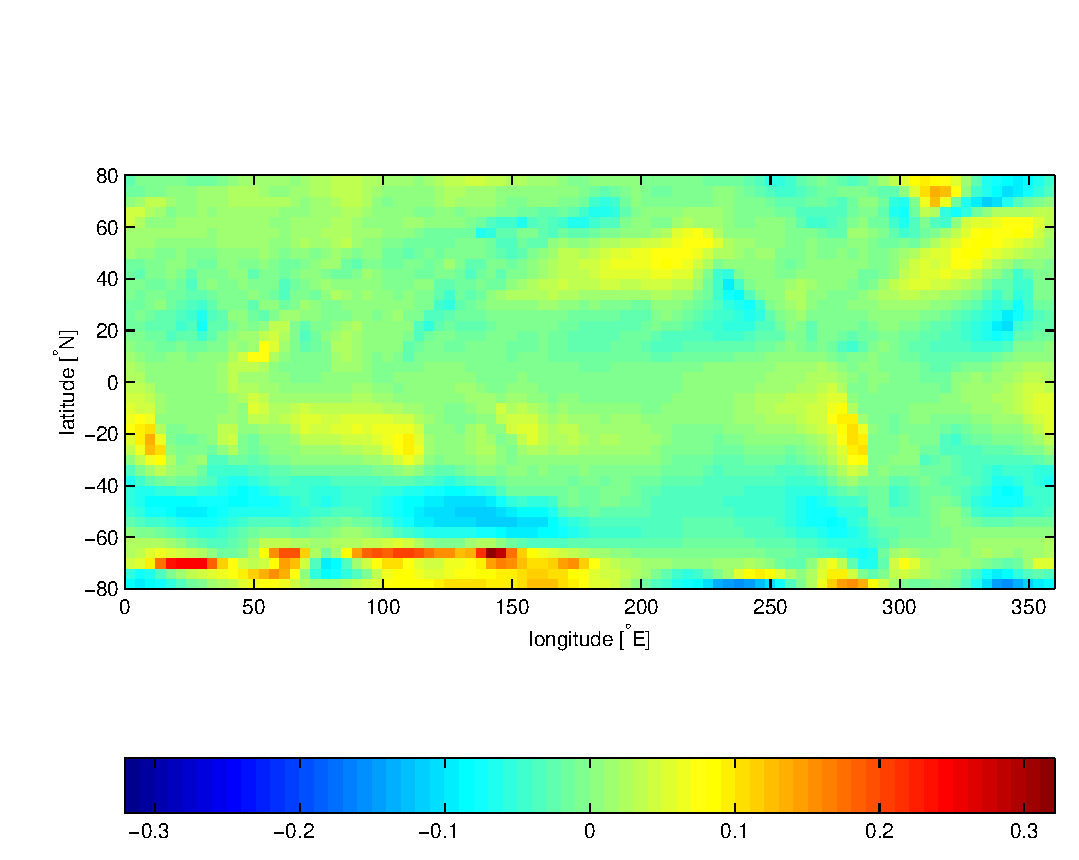
\includegraphics[width=.9\textwidth]{part3/case_studies/ogcm_in_pressure/ty}
    \caption{Annual mean of meridional wind stress component [Nm\,m$^{-2}$]}
    \label{FIG:sim_config_tauy_pcoord}
  \end{center}
\end{figure}
\begin{figure}[t]
  \begin{center}
    \includegraphics[width=.9\textwidth]{part3/case_studies/ogcm_in_pressure/qnet}
    \caption{Annual mean heat flux [W\,m$^{-2}$]}
    \label{FIG:sim_config_qnet_pcoord}
  \end{center}
\end{figure}
\begin{figure}[t]
  \begin{center}
    \includegraphics[width=.9\textwidth]{part3/case_studies/ogcm_in_pressure/emp}
    \caption{Annual mean fresh water flux (Evaporation-Precipitation) [m\,s$^{-1}$]}
    \label{FIG:sim_config_empmr_pcoord}
  \end{center}
\end{figure}
\begin{figure}[t]
  \begin{center}
    \includegraphics[width=.9\textwidth]{part3/case_studies/ogcm_in_pressure/pb0}
    \caption{Model bathymetry in pressure units [Pa]}
    \label{FIG:model_bathymetry_pcoord}
  \end{center}
\end{figure}

\subsubsection{File {\it input/data}}
\label{www:tutorials}

This file, reproduced completely below, specifies the main parameters 
for the experiment. The parameters that are significant for this configuration
are

\begin{itemize}

\item Line 15, 
\begin{verbatim} viscAr=1.721611620915750E+05, \end{verbatim}
this line sets the vertical Laplacian dissipation coefficient to
$1.72161162091575 \times 10^{5} {\rm Pa^{2}s^{-1}}$. Note that, the factor
$(g\rho)^2$ needs to be included in this line. Boundary conditions
for this operator are specified later. This variable is copied into
model general vertical coordinate variable {\bf viscAr}.

\fbox{
\begin{minipage}{5.0in}
{\it S/R CALC\_DIFFUSIVITY}({\it calc\_diffusivity.F})
\end{minipage}
}

\item Line 9--10, 
\begin{verbatim}
viscAh=3.E5,
no_slip_sides=.TRUE.
\end{verbatim} 
  these lines set the horizontal Laplacian frictional dissipation
  coefficient to $3 \times 10^{5} {\rm m^{2}s^{-1}}$ and specify a
  no-slip boundary condition for this operator, that is, $u=0$ along
  boundaries in $y$ and $v=0$ along boundaries in $x$.

\item Lines 11-13,
\begin{verbatim}
 viscAr =1.721611620915750e5,
#viscAz =1.67E-3,
 no_slip_bottom=.FALSE.,
\end{verbatim}
  These lines set the vertical Laplacian frictional dissipation
  coefficient to $1.721611620915750 \times
  10^{5}\mbox{\,Pa$^{2}$s$^{-1}$}$, which corresponds to
  $1.67\times10^{-3}\mbox{\,m$^{2}$s$^{-1}$}$ in the commented line, and
  specify a free slip boundary condition for this operator, that is,
  $\frac{\partial u}{\partial p}=\frac{\partial v}{\partial p}=0$ at
  $p=p_{b}^{0}$, where $p_{b}^{0}$ is the local bottom pressure of the
  domain at rest. Note that, the factor $(g\rho)^2$ needs to be
  included in this line.

\item Line 14,
\begin{verbatim}
 diffKhT=1.E3,
\end{verbatim}
  this line sets the horizontal diffusion coefficient for temperature
  to $1000\,{\rm m^{2}s^{-1}}$. The boundary condition on this
  operator is $\frac{\partial}{\partial x}=\frac{\partial}{\partial
    y}=0$ on all boundaries.

\item Line 15--16,
\begin{verbatim}
 diffKrT=5.154525811125000e3,
#diffKzT=0.5E-4,
\end{verbatim}
  this line sets the vertical diffusion coefficient for temperature to
  $5.154525811125 \times 10^{3}\,{\rm Pa^{2}s^{-1}}$, which
  corresponds to $5\times10^{-4}\mbox{\,m$^{2}$s$^{-1}$}$ in the commented
  line. Note that, the factor $(g\rho)^2$ needs to be included in this
  line. The boundary condition on this operator is
  $\frac{\partial}{\partial p}=0$ at both the upper and lower
  boundaries.

\item Line 17--19,
\begin{verbatim}
 diffKhS=1.E3,
 diffKrS=5.154525811125000e3,
#diffKzS=0.5E-4,
\end{verbatim}
These lines set the same values for the diffusion coefficients for
salinity as for temperature.

\item Line 20--22,
\begin{verbatim}
 implicitDiffusion=.TRUE.,
 ivdc_kappa=1.030905162225000E9,
#ivdc_kappa=10.0,
\end{verbatim}
Select implicit diffusion as a convection scheme and set coefficient
for implicit vertical diffusion to $1.030905162225\times10^{9}\,{\rm
  Pa^{2}s^{-1}}$, which corresponds to $10\mbox{\,m$^{2}$\,s$^{-1}$}$.

\item Line 23-24,
\begin{verbatim}
 gravity=9.81,
 gravitySign=-1.D0,
\end{verbatim}
  These lines set the gravitational acceleration coefficient to
  $9.81{\rm m}{\rm s}^{-1}$ and define the upward direction relative
  to the direction of increasing vertical coordinate (in pressure
  coordinates, up is in the direction of decreasing pressure)
\item Line 25,
\begin{verbatim}
 rhoNil=1035.,
\end{verbatim}
  sets the reference density of sea water to $1035\mbox{\,kg\,m$^{-3}$}$.\\
\fbox{
\begin{minipage}{5.0in}
{\it S/R CALC\_PHI\_HYD}~({\it calc\_phi\_hyd.F})\\
{\it S/R INI\_CG2D}~({\it ini\_cg2d.F})\\
{\it S/R INI\_CG3D}~({\it ini\_cg3d.F})\\
{\it S/R INI\_PARMS}~({\it ini\_parms.F})\\
{\it S/R SOLVE\_FOR\_PRESSURE}~({\it solve\_for\_pressure.F})
\end{minipage}
}

\item Line 28
\begin{verbatim}
 eosType='JMD95P',
\end{verbatim}
  Selects the full equation of state according to Jackett and McDougall
  \cite{jackett95}. The only other sensible choice is the equation of
  state by McDougall et al. \cite{mcdougall03}, 'MDJFW'. All other
  equations of state do not make sense in this configuration.\\
  \fbox{
    \begin{minipage}{5.0in}
      {\it S/R FIND\_RHO}~({\it find\_rho.F})\\
      {\it S/R FIND\_ALPHA}~({\it find\_alpha.F})
    \end{minipage}
    }

\item Line 28-29,
\begin{verbatim}
 rigidLid=.FALSE., 
 implicitFreeSurface=.TRUE., 
\end{verbatim}
  Selects the barotropic pressure equation to be the implicit free
  surface formulation.
\item Line 30
\begin{verbatim}
 exactConserv=.TRUE.,
\end{verbatim}
  Select a more accurate conservation of properties at the surface
  layer by including the horizontal velocity divergence to update the
  free surface.
\item Line 31--33
\begin{verbatim}
 nonlinFreeSurf=3,
 hFacInf=0.2,
 hFacSup=2.0,
\end{verbatim}
  Select the nonlinear free surface formulation and set lower and
  upper limits for the free surface excursions.
\item Line 34
\begin{verbatim}
 useRealFreshWaterFlux=.FALSE.,
\end{verbatim}
  Select virtual salt flux boundary condition for salinity. The
  freshwater flux at the surface only affect the surface salinity, but 
  has no mass flux associated with it

\item Line 35--36,
\begin{verbatim}
 readBinaryPrec=64,
 writeBinaryPrec=64,
\end{verbatim}
  Sets format for reading binary input datasets and 
  writing binary output datasets holding model fields to
  use 64-bit representation for floating-point numbers.\\
  \fbox{
    \begin{minipage}{5.0in}
      {\it S/R READ\_WRITE\_FLD}~({\it read\_write\_fld.F})\\
      {\it S/R READ\_WRITE\_REC}~({\it read\_write\_rec.F})
    \end{minipage}
    }

\item Line 42,
\begin{verbatim}
 cg2dMaxIters=200,
\end{verbatim}
  Sets maximum number of iterations the two-dimensional, conjugate
  gradient solver will use, {\bf irrespective of convergence 
    criteria being met}.\\
  \fbox{
    \begin{minipage}{5.0in}
      {\it S/R CG2D}~({\it cg2d.F})
    \end{minipage}
    }

\item Line 43,
\begin{verbatim}
cg2dTargetResidual=1.E-13,
\end{verbatim}
  Sets the tolerance which the two-dimensional, conjugate
  gradient solver will use to test for convergence in equation 
  \ref{EQ:congrad_2d_resid} to $1 \times 10^{-9}$.
  Solver will iterate until 
  tolerance falls below this value or until the maximum number of
  solver iterations is reached.\\
  \fbox{
    \begin{minipage}{5.0in}
      {\it S/R CG2D}~({\it cg2d.F})
    \end{minipage}
    }

\item Line 48,
\begin{verbatim}
startTime=0,
\end{verbatim}
Sets the starting time for the model internal time counter.
When set to non-zero this option implicitly requests a 
checkpoint file be read for initial state.
By default the checkpoint file is named according to
the integer number of time steps in the {\bf startTime} value.
The internal time counter works in seconds.

\item Line 49--50,
\begin{verbatim}
 endTime=8640000.,
#endTime=62208000000,
\end{verbatim}
  Sets the time (in seconds) at which this simulation will terminate.
  At the end of a simulation a checkpoint file is automatically
  written so that a numerical experiment can consist of multiple
  stages.  The commented out setting for endTime is for a 2000 year
  simulation.

\item Line 51--53,
\begin{verbatim}
 deltaTmom      =   1200.0,
 deltaTtracer   = 172800.0,
 deltaTfreesurf = 172800.0,
\end{verbatim}
  Sets the timestep $\delta t_{v}$ used in the momentum equations to
  $20~{\rm mins}$ and the timesteps $\delta t_{\theta}$ in the tracer
  equations and $\delta t_{\eta}$ in the implicit free surface
  equation to $48\mbox{\,hours}$.  See section
  \ref{SEC:mom_time_stepping}.\\
\fbox{
\begin{minipage}{5.0in}
{\it S/R TIMESTEP}({\it timestep.F}) \\
{\it S/R INI\_PARMS}({\it ini\_parms.F})\\
{\it S/R CALC\_MOM\_RHS}({\it calc\_mom\_rhs.F}) \\
{\it S/R TIMESTEP\_TRACER}({\it timestep\_tracer.F})
\end{minipage}
}

\item Line 55,
\begin{verbatim}
 pChkptFreq  =3110400000.,
\end{verbatim}
write a pick-up file every 100 years of integration.

\item Line 56--58
\begin{verbatim}
 dumpFreq    = 3110400000.,
 taveFreq    = 3110400000.,
 monitorFreq =   31104000.,
\end{verbatim}
  write model output and time-averaged model output every 100 years,
  and monitor statisitics every year.

\item Line 59--61
\begin{verbatim}
 periodicExternalForcing=.TRUE.,
 externForcingPeriod=2592000.,
 externForcingCycle=31104000.,
\end{verbatim}
  Allow periodic external forcing, set forcing period, during which
  one set of data is valid, to 1 month and the repeat cycle to 1 year.\\
\fbox{
\begin{minipage}{5.0in}
{\it S/R EXTERNAL\_FORCING\_SURF}({\it external\_forcing\_surf.F})
\end{minipage}
}
\item Line 62
\begin{verbatim}
 tauThetaClimRelax=5184000.0,
\end{verbatim}
  Set the restoring timescale to 2 months.\\
\fbox{
\begin{minipage}{5.0in}
{\it S/R EXTERNAL\_FORCING\_SURF}({\it external\_forcing\_surf.F})
\end{minipage}
}

\item Line 63
\begin{verbatim}
 abEps=0.1,
\end{verbatim}
  Adams-Bashford factor (see section \ref{sect:adams-bashforth})

\item Line 68--69
\begin{verbatim}
 usingCartesianGrid=.FALSE.,
 usingSphericalPolarGrid=.TRUE.,
\end{verbatim}
  Select spherical grid.
\item Line 70--71
\begin{verbatim}
 dXspacing=4.,
 dYspacing=4.,
\end{verbatim}
Set the horizontal grid spacing in degrees spherical distance.
\item Line 72
\begin{verbatim}
 Ro_SeaLevel=53023122.566084,
\end{verbatim}
specifies the total height (in $r$-units, i.e., pressure units) of the
sea surface at rest. This is a reference value.
\item Line 73
\begin{verbatim}
 groundAtK1=.TRUE.,
\end{verbatim}
specifies the reversal of the vertical indexing. The vertical index is 
1 at the bottom of the doman and maximal (i.e., 15) at the surface.
\item Line 74--78
\begin{verbatim}
 delR=7103300.720021, \ldots 
\end{verbatim}
  set the layer thickness in pressure units, starting with the bottom
  layer.

\item Line 84--93,
\begin{verbatim}
 bathyFile='topog.box'
 ploadFile='deltageopotjmd95.bin'
 hydrogThetaFile='lev_t.bin',
 hydrogSaltFile ='lev_s.bin',
 zonalWindFile  ='trenberth_taux.bin',
 meridWindFile  ='trenberth_tauy.bin',
 thetaClimFile  ='lev_sst.bin',
 surfQFile      ='shi_qnet.bin',
 EmPmRFile      ='shi_empmr.bin',
\end{verbatim}
  This line specifies the names of the files holding the bathymetry
  data set, the
  time-independent geopotential height anomaly at the bottom, initial
  conditions of temperature and salinity, wind stress forcing fields,
  sea surface temperature climatology, heat flux, and fresh water flux
  (evaporation minus precipitation minus run-off) at the surface. 
  See file descriptions in section \ref{SEC:eg-globalpressure-config}.

\end{itemize}

\noindent other lines in the file {\it input/data} are standard values
that are described in the MITgcm Getting Started and MITgcm Parameters
notes.

\begin{small}
% $Header: /u/gcmpack/manual/s_examples/baroclinic_gyre/input/data.tex,v 1.1.1.1 2001/08/08 16:15:46 adcroft Exp $
% $Name:  $

\begin{verbatim}
     1	# Model parameters
     2	# Continuous equation parameters
     3	 &PARM01
     4	 tRef=20.,10.,8.,6.,
     5	 sRef=10.,10.,10.,10.,
     6	 viscAz=1.E-2,
     7	 viscAh=4.E2,
     8	 no_slip_sides=.FALSE.,
     9	 no_slip_bottom=.TRUE.,
    10	 diffKhT=4.E2,
    11	 diffKzT=1.E-2,
    12	 beta=1.E-11,
    13	 tAlpha=2.E-4,
    14	 sBeta =0.,
    15	 gravity=9.81,
    16	 rigidLid=.FALSE.,
    17	 implicitFreeSurface=.TRUE.,
    18	 eosType='LINEAR',
    19	 readBinaryPrec=64,
    20	 &
    21	# Elliptic solver parameters
    22	 &PARM02
    23	 cg2dMaxIters=1000,
    24	 cg2dTargetResidual=1.E-13,
    25	 &
    26	# Time stepping parameters
    27	 &PARM03
    28	 startTime=0.,
    29	 endTime=12000., 
    30	 deltaTmom=1200.0,
    31	 deltaTtracer=1200.0,
    32	 abEps=0.1,
    33	 pChkptFreq=17000.0,
    34	 chkptFreq=0.0,
    35	 dumpFreq=2592000.0,
    36	 &
    37	# Gridding parameters
    38	 &PARM04
    39	 usingCartesianGrid=.FALSE.,
    40	 usingSphericalPolarGrid=.TRUE.,
    41	 phiMin=0.,
    42	 delX=60*1.,
    43	 delY=60*1.,
    44	 delZ=500.,500.,500.,500.,
    45	 &
    46	 &PARM05
    47	 bathyFile='topog.box',
    48	 hydrogThetaFile=,
    49	 hydrogSaltFile=,
    50	 zonalWindFile='windx.sin_y',
    51	 meridWindFile=,
    52	 &
\end{verbatim}

\end{small}

\subsubsection{File {\it input/data.pkg}}
\label{www:tutorials}

This file uses standard default values and does not contain
customisations for this experiment.

\subsubsection{File {\it input/eedata}}
\label{www:tutorials}

This file uses standard default values and does not contain
customisations for this experiment.

\subsubsection{File {\it input/topog.bin}}
\label{www:tutorials}

This file is a two-dimensional ($x,y$) map of
depths. This file is assumed to contain 64-bit binary numbers giving
the depth of the model at each grid cell, ordered with the x
coordinate varying fastest. The points are ordered from low
coordinate to high coordinate for both axes. The units and
orientation of the depths in this file are the same as used in the
MITgcm code (Pa for this experiment). In this experiment, a depth of
$0\mbox{\,Pa}$ indicates a land point wall and a depth of
$>0\mbox{\,Pa}$ indicates open ocean.

\subsubsection{File {\it input/deltageopotjmd95.box}}
\label{www:tutorials}

The file contains 12 identical two dimensional maps ($x,y$) of
geopotential height anomaly at the bottom at rest. The values have
been obtained by vertically integrating the hydrostatic equation with
the initial density field (from {\it input/lev\_t/s.bin}). This file
has to be consitent with the temperature and salinity field at rest
and the choice of equation of state!

\subsubsection{File {\it input/lev\_t/s.bin}}
\label{www:tutorials}

The files {\it input/lev\_t/s.bin} specify the initial conditions for
temperature and salinity for every grid point in a three dimensional
array ($x,y,z$). The data are obtain by interpolating Levitus
\cite{Levitus94} monthly mean values for January onto the model
grid. Keep in mind, that the first index corresponds to the bottom
layer and highest index to the surface layer.

\subsubsection{File {\it input/trenberth\_taux/y.bin}}
\label{www:tutorials}

Each of the {\it input/trenberth\_taux/y.bin} files specifies 12
two-dimensional ($x,y,t$) maps of zonal and meridional wind stress
values, $\tau_{x}$ and $\tau_{y}$, that is monthly mean values from
Trenberth \cite{trenberth90}. The units used are $Nm^{-2}$.

\subsubsection{File {\it input/lev\_sst.bin}}
\label{www:tutorials}

The file {\it input/lev\_sst.bin} contains 12 monthly surface
temperature climatologies from Levitus \cite{Levitus94} in a three
dimensional array ($x,y,t$).

\subsubsection{File {\it input/shi\_qnet/empmr.bin}}
\label{www:tutorials}

The files {\it input/shi\_qnet/empmr.bin} contain 12 monthly surface
fluxes of heat (qnet) and freshwater (empmr) by Jiang et al.
\cite{jiang99} in three dimensional arrays ($x,y,t$). Both fluxes are
normalized so that of one year there is no net flux into the
ocean. The freshwater flux is actually constant in time.

\subsubsection{File {\it code/SIZE.h}}
\label{www:tutorials}

Three lines are customized in this file for the current experiment

\begin{itemize}

\item Line 39, 
\begin{verbatim} sNx=90, \end{verbatim} this line sets
the lateral domain extent in grid points for the
axis aligned with the x-coordinate.

\item Line 40, 
\begin{verbatim} sNy=40, \end{verbatim} this line sets
the lateral domain extent in grid points for the
axis aligned with the y-coordinate.

\item Line 49, 
\begin{verbatim} Nr=15,   \end{verbatim} this line sets
the vertical domain extent in grid points.

\end{itemize}

\begin{small}
% $Header: /u/gcmpack/manual/s_examples/barotropic_gyre/code/SIZE.h.tex,v 1.1.1.1 2001/08/08 16:15:58 adcroft Exp $
% $Name:  $

\begin{verbatim}
     1	C $Header: /u/gcmpack/manual/s_examples/barotropic_gyre/code/SIZE.h.tex,v 1.1.1.1 2001/08/08 16:15:58 adcroft Exp $
     2	C $Name:  $
     3	C
     4	C     /==========================================================\
     5	C     | SIZE.h Declare size of underlying computational grid.    |
     6	C     |==========================================================|
     7	C     | The design here support a three-dimensional model grid   |
     8	C     | with indices I,J and K. The three-dimensional domain     |
     9	C     | is comprised of nPx*nSx blocks of size sNx along one axis|
    10	C     | nPy*nSy blocks of size sNy along another axis and one    |
    11	C     | block of size Nz along the final axis.                   |
    12	C     | Blocks have overlap regions of size OLx and OLy along the|
    13	C     | dimensions that are subdivided.                          |
    14	C     \==========================================================/
    15	C     Voodoo numbers controlling data layout.
    16	C     sNx - No. X points in sub-grid.
    17	C     sNy - No. Y points in sub-grid.
    18	C     OLx - Overlap extent in X.
    19	C     OLy - Overlat extent in Y.
    20	C     nSx - No. sub-grids in X.
    21	C     nSy - No. sub-grids in Y.
    22	C     nPx - No. of processes to use in X.
    23	C     nPy - No. of processes to use in Y.
    24	C     Nx  - No. points in X for the total domain.
    25	C     Ny  - No. points in Y for the total domain.
    26	C     Nr  - No. points in R for full process domain.
    27	      INTEGER sNx
    28	      INTEGER sNy
    29	      INTEGER OLx
    30	      INTEGER OLy
    31	      INTEGER nSx
    32	      INTEGER nSy
    33	      INTEGER nPx
    34	      INTEGER nPy
    35	      INTEGER Nx
    36	      INTEGER Ny
    37	      INTEGER Nr
    38	      PARAMETER (
    39	     &           sNx =  60,
    40	     &           sNy =  60,
    41	     &           OLx =   3,
    42	     &           OLy =   3,
    43	     &           nSx =   1,
    44	     &           nSy =   1,
    45	     &           nPx =   1,
    46	     &           nPy =   1,
    47	     &           Nx  = sNx*nSx*nPx,
    48	     &           Ny  = sNy*nSy*nPy,
    49	     &           Nr  =   1)
       
    50	C     MAX_OLX  - Set to the maximum overlap region size of any array
    51	C     MAX_OLY    that will be exchanged. Controls the sizing of exch
    52	C                routine buufers.
    53	      INTEGER MAX_OLX
    54	      INTEGER MAX_OLY
    55	      PARAMETER ( MAX_OLX = OLx,
    56	     &            MAX_OLY = OLy )
\end{verbatim}

\end{small}

\subsubsection{File {\it code/CPP\_OPTIONS.h}}
\label{www:tutorials}

This file uses mostly standard default values except for:
\begin{itemize}
\item \verb+#define ATMOSPHERIC_LOADING+\\
  enable pressure loading which is abused to include the initial
  geopotential height anomaly
\item \verb+#define EXACT_CONSERV+\\
  enable more accurate conservation properties to include the
  horizontal mass divergence in the free surface 
\item \verb+#define NONLIN_FRSURF+\\
  enable the nonlinear free surface
\end{itemize}


\subsubsection{File {\it code/CPP\_EEOPTIONS.h}}
\label{www:tutorials}

This file uses standard default values and does not contain
customisations for this experiment.




\newpage
\input{part3/case_studies/hs_atmosphere/hs_atmos.tex}

\newpage
\section{Example: Surface driven convection}
\label{sect:eg-bconv}

\bodytext{bgcolor="#FFFFFFFF"}

%\begin{center} 
%{\Large \bf Surface driven convection}
%
%\vspace*{4mm}
%
%\vspace*{3mm}
%{\large Dec 2001}
%\end{center}

\begin{figure}
\begin{center}
 \resizebox{7.5cm}{5.5cm}{
   \includegraphics*[0.2in,0.7in][10.5in,10.5in]
   {part3/case_studies/doubly_periodic_convection/simulation_config.eps} }
\end{center}
\caption{Schematic of simulation domain 
for the surface driven convection experiment. The domain is doubly periodic
with an initially uniform temperature of 20 $^oC$. 
}
\label{FIG:simulation_config}
\end{figure}

This experiment, figure \ref{FIG:simulation_config}, showcasing MITgcm's non-hydrostatic capability, was designed to explore 
the temporal and spatial characteristics of convection plumes as they might exist during a 
period of oceanic deep convection. It is

\begin{itemize}
\item non-hydrostatic 
\item doubly-periodic with cubic geometry
\item has 50 m resolution 
\item Cartesian  
\item is on an $f$-plane 
\item with a linear equation of state 
\end{itemize}

\subsection{Overview}

The model domain consists of an approximately 3
km square by 1 km deep box of initially
unstratified, resting fluid. The domain is doubly periodic. 

The experiment has 20 levels in the vertical, each of equal thickness $\Delta z =$ 50
m (the horizontal resolution is also 50 m). The fluid is initially unstratified with a
uniform reference potential temperature $\theta = $ 20 $^o$C. The equation of state
used in this experiment is linear

\begin{equation}
\label{EQ:linear1_eos}
\rho = \rho_{0} ( 1 - \alpha_{\theta}\theta^{'} )
\end{equation}

\noindent which is implemented in the model as a density anomaly equation

\begin{equation}
\label{EQ:linear1_eos_pert}
\rho^{'} = -\rho_{0}\alpha_{\theta}\theta^{'}
\end{equation}

\noindent with $\rho_{0}=1000\,{\rm kg\,m}^{-3}$ and 
$\alpha_{\theta}=2\times10^{-4}\,{\rm degrees}^{-1} $. Integrated forward in
this configuration the model state variable {\bf theta} is equivalent to
either in-situ temperature, $T$, or potential temperature, $\theta$. For 
consistency with other examples, in which the equation of state is
non-linear, we use $\theta$ to represent temperature here. This is
the quantity that is carried in the model core equations.

As the fluid in the surface layer is cooled (at a mean rate of 800 Wm$^2$), it becomes 
convectively unstable and 
overturns, at first close to the grid-scale, but, as the flow matures, on larger scales 
(figures \ref{FIG:vertsection} and \ref{FIG:horizsection}), under the influence of 
rotation ($f_o = 10^{-4}$ s$^{-1}$) .

\begin{figure}
\begin{center}
 \resizebox{15cm}{10cm}{
   \includegraphics*[0.2in,0.7in][10.5in,10.5in]
   {part3/case_studies/doubly_periodic_convection/verticalsection.ps} }
\end{center}
\caption{
}
\label{FIG:vertsection}
\end{figure}

\begin{figure}
\begin{center}
 \resizebox{10cm}{10cm}{
   \includegraphics*[0.2in,0.7in][10.5in,10.5in]
   {part3/case_studies/doubly_periodic_convection/surfacesection.ps} }
\end{center}
\caption{
}
\label{FIG:horizsection}
\end{figure}

Model parameters are specified in file {\it input/data}. The grid dimensions are
prescribed in {\it code/SIZE.h}. The forcing (file {\it input/Qsurf.bin}) is specified 
in a binary data file generated using the Matlab script {\it input/gendata.m}.

\subsection{Equations solved}

The model is configured in nonhydrostatic form, that is, all terms in the Navier 
Stokes equations are retained and the pressure field is found, subject to appropriate
bounday condintions, through inversion of a three-dimensional elliptic equation. 

The implicit free surface form of the
pressure equation described in Marshall et. al \cite{marshall:97a} is
employed. A horizontal Laplacian operator $\nabla_{h}^2$ provides viscous
dissipation. The thermodynamic forcing appears as a sink in the potential temperature, 
$\theta$, equation (\ref{EQ:global_forcing_ft}). This produces a set of equations 
solved in this configuration as follows:

\begin{eqnarray}
\label{EQ:model_equations}
\frac{Du}{Dt} - fv + 
  \frac{1}{\rho}\frac{\partial p^{'}}{\partial x} - 
  \nabla_{h}\cdot A_{h}\nabla_{h}u - 
  \frac{\partial}{\partial z}A_{z}\frac{\partial u}{\partial z} 
 & = &
\begin{cases}
0 & \text{(surface)} \\
0 & \text{(interior)}
\end{cases}
\\
\frac{Dv}{Dt} + fu + 
  \frac{1}{\rho}\frac{\partial p^{'}}{\partial y} - 
  \nabla_{h}\cdot A_{h}\nabla_{h}v - 
  \frac{\partial}{\partial z}A_{z}\frac{\partial v}{\partial z} 
& = &
\begin{cases}
0 & \text{(surface)} \\
0 & \text{(interior)}
\end{cases}
\\
\frac{Dw}{Dt} + g \frac{\rho^{'}}{\rho} + 
  \frac{1}{\rho}\frac{\partial p^{'}}{\partial z} - 
  \nabla_{h}\cdot A_{h}\nabla_{h}w - 
  \frac{\partial}{\partial z}A_{z}\frac{\partial w}{\partial z} 
& = &
\begin{cases}
0 & \text{(surface)} \\
0 & \text{(interior)}
\end{cases}
\\
\frac{\partial u}{\partial x} + 
\frac{\partial v}{\partial y} + 
\frac{\partial w}{\partial z} + 
&=&
0
\\
\frac{D\theta}{Dt} -
 \nabla_{h}\cdot K_{h}\nabla_{h}\theta
 - \frac{\partial}{\partial z}K_{z}\frac{\partial\theta}{\partial z} 
& = &
\begin{cases}
{\cal F}_\theta & \text{(surface)} \\
0 & \text{(interior)}
\end{cases}
\end{eqnarray}

\noindent where $u=\frac{Dx}{Dt}$, $v=\frac{Dy}{Dt}$  and 
$w=\frac{Dz}{Dt}$ are the components of the
flow vector in directions $x$, $y$ and $z$. 
The pressure is diagnosed through inversion (subject to appropriate boundary
conditions) of a 3-D elliptic equation derived from the divergence of the momentum 
equations and continuity (see section \ref{sec:finding_the_pressure_field}).
\\

\subsection{Discrete numerical configuration}

The domain is discretised with a uniform grid spacing in each direction. There are 64
grid cells in directions $x$ and $y$ and 20 vertical levels thus the domain
comprises a total of just over 80 000 gridpoints.

\subsection{Numerical stability criteria and other considerations}

For a heat flux of 800 Wm$^2$ and a rotation rate of $10^{-4}$ s$^{-1}$ the
plume-scale can be expected to be a few hundred meters guiding our choice of grid
resolution. This in turn restricts the timestep we can take. It is also desirable to 
minimise the level of diffusion and viscosity we apply.

For this class of problem it is generally the advective time-scale which restricts 
the timestep. 

For an extreme maximum flow speed of $ | \vec{u} | = 1 ms^{-1}$, at a resolution of
50 m, the implied maximum timestep for stability, $\delta t_u$ is 

\begin{eqnarray}
\label{EQ:advectiveCFLcondition}
%\delta t_u = \frac{\Delta x}{| \vec{u} \} = 50 s
\end{eqnarray}

The choice of $\delta t = 10$ s is a safe 20 percent of this maximum.
 
Interpreted in terms of a mixing-length hypothesis, a magnitude of Laplacian
diffusion coefficient $\kappa_h (=
\kappa_v) = 0.1$ m$^2$s$^{-1}$ is consistent with an eddy velocity of 2 mm s$^{-1}$
correlated over 50 m.  

\subsection{Experiment configuration}

The model configuration for this experiment resides under the directory
{\it verification/convection/}. The experiment files
\begin{itemize}
\item {\it code/CPP\_EEOPTIONS.h}
\item {\it code/CPP\_OPTIONS.h},
\item {\it code/SIZE.h}. 
\item {\it input/data}
\item {\it input/data.pkg}
\item {\it input/eedata},
\item {\it input/Qsurf.bin},
\end{itemize}
contain the code customisations and parameter settings for this 
experiment. Below we describe these experiment-specific customisations.

\subsubsection{File {\it code/CPP\_EEOPTIONS.h}}

This file uses standard default values and does not contain
customisations for this experiment.

\subsubsection{File {\it code/CPP\_OPTIONS.h}}

This file uses standard default values and does not contain
customisations for this experiment.

\subsubsection{File {\it code/SIZE.h}}

Three lines are customized in this file. These prescribe the domain grid dimensions.
\begin{itemize}

\item Line 36, 
\begin{verbatim} sNx=64, \end{verbatim} this line sets
the lateral domain extent in grid points for the
axis aligned with the $x$-coordinate.

\item Line 37, 
\begin{verbatim} sNy=64, \end{verbatim} this line sets
the lateral domain extent in grid points for the
axis aligned with the $y$-coordinate.

\item Line 46, 
\begin{verbatim} Nr=20,   \end{verbatim} this line sets
the vertical domain extent in grid points.

\end{itemize}

\begin{rawhtml}<PRE>\end{rawhtml}
\begin{small}
% $Header: /u/gcmpack/manual/s_examples/barotropic_gyre/code/SIZE.h.tex,v 1.1.1.1 2001/08/08 16:15:58 adcroft Exp $
% $Name:  $

\begin{verbatim}
     1	C $Header: /u/gcmpack/manual/s_examples/barotropic_gyre/code/SIZE.h.tex,v 1.1.1.1 2001/08/08 16:15:58 adcroft Exp $
     2	C $Name:  $
     3	C
     4	C     /==========================================================\
     5	C     | SIZE.h Declare size of underlying computational grid.    |
     6	C     |==========================================================|
     7	C     | The design here support a three-dimensional model grid   |
     8	C     | with indices I,J and K. The three-dimensional domain     |
     9	C     | is comprised of nPx*nSx blocks of size sNx along one axis|
    10	C     | nPy*nSy blocks of size sNy along another axis and one    |
    11	C     | block of size Nz along the final axis.                   |
    12	C     | Blocks have overlap regions of size OLx and OLy along the|
    13	C     | dimensions that are subdivided.                          |
    14	C     \==========================================================/
    15	C     Voodoo numbers controlling data layout.
    16	C     sNx - No. X points in sub-grid.
    17	C     sNy - No. Y points in sub-grid.
    18	C     OLx - Overlap extent in X.
    19	C     OLy - Overlat extent in Y.
    20	C     nSx - No. sub-grids in X.
    21	C     nSy - No. sub-grids in Y.
    22	C     nPx - No. of processes to use in X.
    23	C     nPy - No. of processes to use in Y.
    24	C     Nx  - No. points in X for the total domain.
    25	C     Ny  - No. points in Y for the total domain.
    26	C     Nr  - No. points in R for full process domain.
    27	      INTEGER sNx
    28	      INTEGER sNy
    29	      INTEGER OLx
    30	      INTEGER OLy
    31	      INTEGER nSx
    32	      INTEGER nSy
    33	      INTEGER nPx
    34	      INTEGER nPy
    35	      INTEGER Nx
    36	      INTEGER Ny
    37	      INTEGER Nr
    38	      PARAMETER (
    39	     &           sNx =  60,
    40	     &           sNy =  60,
    41	     &           OLx =   3,
    42	     &           OLy =   3,
    43	     &           nSx =   1,
    44	     &           nSy =   1,
    45	     &           nPx =   1,
    46	     &           nPy =   1,
    47	     &           Nx  = sNx*nSx*nPx,
    48	     &           Ny  = sNy*nSy*nPy,
    49	     &           Nr  =   1)
       
    50	C     MAX_OLX  - Set to the maximum overlap region size of any array
    51	C     MAX_OLY    that will be exchanged. Controls the sizing of exch
    52	C                routine buufers.
    53	      INTEGER MAX_OLX
    54	      INTEGER MAX_OLY
    55	      PARAMETER ( MAX_OLX = OLx,
    56	     &            MAX_OLY = OLy )
\end{verbatim}

\end{small}
\begin{rawhtml}</PRE>\end{rawhtml}

\subsubsection{File {\it input/data}}

This file, reproduced completely below, specifies the main parameters 
for the experiment. The parameters that are significant for this configuration
are

\begin{itemize}

\item Line 4, 
\begin{verbatim}
     4	 tRef=20*20.0,
\end{verbatim}
this line sets
the initial and reference values of potential temperature at each model
level in units of $^{\circ}$C. Here the value is arbitrary since, in this case, the 
flow evolves independently of the absolute magnitude of the reference temperature.
For each depth level the initial and reference profiles will be uniform in
$x$ and $y$. The values specified are read into the
variable 
{\bf 
\begin{rawhtml} <A href=../../../code_reference/vdb/names/OK.htm> \end{rawhtml}
tRef
\begin{rawhtml} </A>\end{rawhtml}
} 
in the model code, by procedure 
{\it
\begin{rawhtml} <A href=../../../code_reference/vdb/code/94.htm> \end{rawhtml}
S/R INI\_PARMS ({\it ini\_parms.F})
\begin{rawhtml} </A>\end{rawhtml}.
}
The temperature field is initialised, by procedure 
{\it
\begin{rawhtml} <A href=../../../code_reference/vdb/code/OK.htm> \end{rawhtml}
S/R INI\_THETA ({\it ini\_theta.F})
\begin{rawhtml} </A>\end{rawhtml}.
}


\item Line 5,
\begin{verbatim}
     5	 sRef=20*35.0,
\end{verbatim}
this line sets the initial and reference values of salinity at each model
level in units of ppt. In this case salinity is set to an (arbitrary) uniform value of 
35.0 ppt. However since, in this example, density is independent of salinity, 
an appropriatly defined initial salinity could provide a useful passive 
tracer. For each depth level the initial and reference profiles will be uniform in
$x$ and $y$. The values specified are read into the
variable 
{\bf
\begin{rawhtml} <A href=../../../code_reference/vdb/names/OK.htm> \end{rawhtml}
sRef
\begin{rawhtml} </A>\end{rawhtml}
} 
in the model code, by procedure 
{\it
\begin{rawhtml} <A href=../../../code_reference/vdb/code/94.htm> \end{rawhtml}
S/R INI\_PARMS ({\it ini\_parms.F})
}
\begin{rawhtml} </A>\end{rawhtml}.
The salinity field is initialised, by procedure 
{\it
\begin{rawhtml} <A href=../../../code_reference/vdb/code/OK.htm> \end{rawhtml}
S/R INI\_SALT ({\it ini\_salt.F})
\begin{rawhtml} </A>\end{rawhtml}.
}


\item Line 6,
\begin{verbatim}
     6	 viscAh=0.1,
\end{verbatim}
this line sets the horizontal laplacian dissipation coefficient to
0.1 ${\rm m^{2}s^{-1}}$. Boundary conditions
for this operator are specified later. 
The variable 
{\bf 
\begin{rawhtml} <A href=../../../code_reference/vdb/names/SI.htm> \end{rawhtml}
viscAh
\begin{rawhtml} </A>\end{rawhtml}
}
is read in the routine
{\it
\begin{rawhtml} <A href=../../../code_reference/vdb/code/94.htm> \end{rawhtml}
S/R INI\_PARMS ({\it ini\_params.F})
\begin{rawhtml} </A>\end{rawhtml}
} and applied in routines 
{\it 
\begin{rawhtml} <A href=../../../code_reference/vdb/code/94.htm> \end{rawhtml}
S/R CALC\_MOM\_RHS ({\it calc\_mom\_rhs.F})
\begin{rawhtml} </A>\end{rawhtml}
} and 
{\it 
\begin{rawhtml} <A href=../../../code_reference/vdb/code/94.htm> \end{rawhtml}
S/R CALC\_GW ({\it calc\_gw.F})
\begin{rawhtml} </A>\end{rawhtml}
}.


\item Line 7,
\begin{verbatim}
     7	 viscAz=0.1,
\end{verbatim}
this line sets the vertical laplacian frictional dissipation coefficient to
0.1 ${\rm m^{2}s^{-1}}$. Boundary conditions
for this operator are specified later.
The variable 
{\bf 
\begin{rawhtml} <A href=../../../code_reference/vdb/names/ZQ.htm> \end{rawhtml}
viscAz
\begin{rawhtml} </A>\end{rawhtml}
}
is read in the routine
{\it
\begin{rawhtml} <A href=../../../code_reference/vdb/code/94.htm> \end{rawhtml}
S/R INI\_PARMS ({\it ini\_parms.F})
\begin{rawhtml} </A>\end{rawhtml}
}
and is copied into model general vertical coordinate variable 
{\bf 
\begin{rawhtml} <A href=../../../code_reference/vdb/names/PF.htm> \end{rawhtml}
viscAr
\begin{rawhtml} </A>\end{rawhtml}
}. At each time step, the viscous term contribution to the momentum equations
is calculated in routine
{\it 
\begin{rawhtml} <A href=../../../code_reference/vdb/code/94.htm> \end{rawhtml}
S/R CALC\_DIFFUSIVITY ({\it calc\_diffusivity.F})
\begin{rawhtml} </A>\end{rawhtml}
}.


\item Line 8,
\begin{verbatim}
no_slip_sides=.FALSE.
\end{verbatim}
this line selects a free-slip lateral boundary condition for
the horizontal laplacian friction operator 
e.g. $\frac{\partial u}{\partial y}$=0 along boundaries in $y$ and
$\frac{\partial v}{\partial x}$=0 along boundaries in $x$.
The variable
{\bf
\begin{rawhtml} <A href=../../../code_reference/vdb/names/UT.htm> \end{rawhtml}
no\_slip\_sides
\begin{rawhtml} </A>\end{rawhtml}
}
is read in the routine
{\it
\begin{rawhtml} <A href=../../../code_reference/vdb/code/94.htm> \end{rawhtml}
S/R INI\_PARMS ({\it ini\_parms.F})
\begin{rawhtml} </A>\end{rawhtml}
} and the boundary condition is evaluated in routine
{\it 
\begin{rawhtml} <A href=../../../code_reference/vdb/code/94.htm> \end{rawhtml}
S/R CALC\_MOM\_RHS ({\it calc\_mom\_rhs.F})
\begin{rawhtml} </A>\end{rawhtml}
}.


\item Lines 9,
\begin{verbatim}
no_slip_bottom=.TRUE.
\end{verbatim}
this line selects a no-slip boundary condition for the bottom
boundary condition in the vertical laplacian friction operator 
e.g. $u=v=0$ at $z=-H$, where $H$ is the local depth of the domain.
The variable
{\bf
\begin{rawhtml} <A href=../../../code_reference/vdb/names/UK.htm> \end{rawhtml}
no\_slip\_bottom
\begin{rawhtml} </A>\end{rawhtml}
}
is read in the routine
{\it
\begin{rawhtml} <A href=../../../code_reference/vdb/code/94.htm> \end{rawhtml}
S/R INI\_PARMS ({\it ini\_parms.F})
\begin{rawhtml} </A>\end{rawhtml}
} and is applied in the routine 
{\it 
\begin{rawhtml} <A href=../../../code_reference/vdb/code/94.htm> \end{rawhtml}
S/R CALC\_MOM\_RHS ({\it calc\_mom\_rhs.F})
\begin{rawhtml} </A>\end{rawhtml}
}.

\item Line 11,
\begin{verbatim}
diffKhT=0.1,
\end{verbatim}
this line sets the horizontal diffusion coefficient for temperature
to 0.1 $\rm m^{2}s^{-1}$. The boundary condition on this
operator is $\frac{\partial}{\partial x}=\frac{\partial}{\partial y}=0$ at
all boundaries.
The variable
{\bf
\begin{rawhtml} <A href=../../../code_reference/vdb/names/RC.htm> \end{rawhtml}
diffKhT
\begin{rawhtml} </A>\end{rawhtml}
}
is read in the routine
{\it
\begin{rawhtml} <A href=../../../code_reference/vdb/code/94.htm> \end{rawhtml}
S/R INI\_PARMS ({\it ini\_parms.F})
\begin{rawhtml} </A>\end{rawhtml}
} and used in routine 
{\it
\begin{rawhtml} <A href=../../../code_reference/vdb/code/94.htm> \end{rawhtml}
S/R CALC\_GT ({\it calc\_gt.F})
\begin{rawhtml} </A>\end{rawhtml}
}.

\item Line 12,
\begin{verbatim}
diffKzT=0.1,
\end{verbatim}
this line sets the vertical diffusion coefficient for temperature
to 0.1 ${\rm m^{2}s^{-1}}$. The boundary condition on this
operator is $\frac{\partial}{\partial z}$ = 0 on all boundaries.
The variable
{\bf
\begin{rawhtml} <A href=../../../code_reference/vdb/names/ZT.htm> \end{rawhtml}
diffKzT
\begin{rawhtml} </A>\end{rawhtml}
}
is read in the routine
{\it
\begin{rawhtml} <A href=../../../code_reference/vdb/code/94.htm> \end{rawhtml}
S/R INI\_PARMS ({\it ini\_parms.F})
\begin{rawhtml} </A>\end{rawhtml}
}.
It is copied into model general vertical coordinate variable
{\bf
\begin{rawhtml} <A href=../../../code_reference/vdb/names/PD.htm> \end{rawhtml}
diffKrT
\begin{rawhtml} </A>\end{rawhtml}
} which is used in routine 
{\it 
\begin{rawhtml} <A href=../../../code_reference/vdb/code/94.htm> \end{rawhtml}
S/R CALC\_DIFFUSIVITY ({\it calc\_diffusivity.F})
\begin{rawhtml} </A>\end{rawhtml}
}.


\item Line 13,
\begin{verbatim}
diffKhS=0.1,
\end{verbatim}
this line sets the horizontal diffusion coefficient for salinity
to 0.1 $\rm m^{2}s^{-1}$. The boundary condition on this
operator is $\frac{\partial}{\partial x}=\frac{\partial}{\partial y}=0$ on
all boundaries.
The variable
{\bf
\begin{rawhtml} <A href=../../../code_reference/vdb/names/RC.htm> \end{rawhtml}
diffKsT
\begin{rawhtml} </A>\end{rawhtml}
}
is read in the routine
{\it
\begin{rawhtml} <A href=../../../code_reference/vdb/code/94.htm> \end{rawhtml}
S/R INI\_PARMS ({\it ini\_parms.F})
\begin{rawhtml} </A>\end{rawhtml}
} and used in routine 
{\it
\begin{rawhtml} <A href=../../../code_reference/vdb/code/94.htm> \end{rawhtml}
S/R CALC\_GS ({\it calc\_gs.F})
\begin{rawhtml} </A>\end{rawhtml}
}.


\item Line 14,
\begin{verbatim}
diffKzS=0.1,
\end{verbatim}
this line sets the vertical diffusion coefficient for temperature
to 0.1 ${\rm m^{2}s^{-1}}$. The boundary condition on this
operator is $\frac{\partial}{\partial z}$ = 0 on all boundaries.
The variable
{\bf
\begin{rawhtml} <A href=../../../code_reference/vdb/names/ZT.htm> \end{rawhtml}
diffKzS
\begin{rawhtml} </A>\end{rawhtml}
}
is read in the routine
{\it
\begin{rawhtml} <A href=../../../code_reference/vdb/code/94.htm> \end{rawhtml}
S/R INI\_PARMS ({\it ini\_parms.F})
\begin{rawhtml} </A>\end{rawhtml}
}.
It is copied into model general vertical coordinate variable
{\bf
\begin{rawhtml} <A href=../../../code_reference/vdb/names/PD.htm> \end{rawhtml}
diffKrS
\begin{rawhtml} </A>\end{rawhtml}
} which is used in routine 
{\it 
\begin{rawhtml} <A href=../../../code_reference/vdb/code/94.htm> \end{rawhtml}
S/R CALC\_DIFFUSIVITY ({\it calc\_diffusivity.F})
\begin{rawhtml} </A>\end{rawhtml}
}.


\item Line 15,
\begin{verbatim}
f0=1E-4,
\end{verbatim}
this line sets the Coriolis parameter to $1 \times 10^{-4}$ s$^{-1}$. 
Since $\beta = 0.0$ this value is then adopted throughout the domain.

 
\item Line 16,
\begin{verbatim}
beta=0.E-11,
\end{verbatim}
this line sets the the variation of Coriolis parameter with latitude to $0$.


\item Line 17,
\begin{verbatim}
tAlpha=2.E-4,
\end{verbatim}
This line sets the thermal expansion coefficient for the fluid
to $2 \times 10^{-4}$ $^o$ C$^{-1}$.
The variable
{\bf
\begin{rawhtml} <A href=../../../code_reference/vdb/names/ZV.htm> \end{rawhtml}
tAlpha 
\begin{rawhtml} </A>\end{rawhtml}
}
is read in the routine
{\it
\begin{rawhtml} <A href=../../../code_reference/vdb/code/94.htm> \end{rawhtml}
S/R INI\_PARMS ({\it ini\_parms.F})
\begin{rawhtml} </A>\end{rawhtml}
}. 
The routine 
{\it
\begin{rawhtml} <A href=../../../code_reference/vdb/code/94.htm> \end{rawhtml}
S/R FIND\_RHO ({\it find\_rho.F})
\begin{rawhtml} </A>\end{rawhtml}
} makes use of {\bf tAlpha}.

\item Line 18,
\begin{verbatim}
sBeta=0,
\end{verbatim}
This line sets the saline expansion coefficient for the fluid
to $0$ consistent with salt's passive role in this example.


\item Line 23-24,
\begin{verbatim}
rigidLid=.FALSE., 
implicitFreeSurface=.TRUE., 
\end{verbatim}
Selects the barotropic pressure equation to be the implicit free surface
formulation.

\item Line 25,
\begin{verbatim}
eosType='LINEAR',
\end{verbatim}
Selects the linear form of the equation of state.


\item Line 26,
\begin{verbatim}
nonHydrostatic=.TRUE.,
\end{verbatim}
Selects for non-hydrostatic code.


\item Line 27,
\begin{verbatim}
readBinaryPrec=64,
\end{verbatim}
Sets format for reading binary input datasets holding model fields to
use 64-bit representation for floating-point numbers.

\item Line 31,
\begin{verbatim}
cg2dMaxIters=1000,
\end{verbatim}
Inactive - the pressure field in a non-hydrostatic simulation is inverted through a 3D
elliptic equation.


\item Line 32,
\begin{verbatim}
cg2dTargetResidual=1.E-9,
\end{verbatim}
Inactive - the pressure field in a non-hydrostatic simulation is inverted through a 3D
elliptic equation.


\item Line 33,
\begin{verbatim}
cg3dMaxIters=40,
\end{verbatim}
This line sets the  maximum number of iterations the three-dimensional, conjugate
gradient solver will use to 40, {\bf irrespective of the convergence 
criteria being met}. Used in routine
{\it
\begin{rawhtml} <A href=../../../code_reference/vdb/code/94.htm> \end{rawhtml}
S/R CG3D ({\it cg3d.F})
\begin{rawhtml} </A>\end{rawhtml}
}. 



\item Line 34,
\begin{verbatim}
cg3dTargetResidual=1.E-9,
\end{verbatim}
Sets the tolerance which the three-dimensional, conjugate
gradient solver will use to test for convergence in equation 
\ref{EQ:congrad_3d_resid} to $1 \times 10^{-9}$.
The solver will iterate until the 
tolerance falls below this value or until the maximum number of
solver iterations is reached. Used in routine
{\it
\begin{rawhtml} <A href=../../../code_reference/vdb/code/94.htm> \end{rawhtml}
S/R CG3D ({\it cg3d.F})
\begin{rawhtml} </A>\end{rawhtml}
}. 


\item Line 38,
\begin{verbatim}
startTime=0,
\end{verbatim}
Sets the starting time for the model internal time counter.
When set to non-zero this option implicitly requests a 
checkpoint file be read for initial state.
By default the checkpoint file is named according to
the integer number of time steps in the {\bf startTime} value.
The internal time counter works in seconds.

\item Line 39,
\begin{verbatim}
nTimeSteps=8640.,
\end{verbatim}
Sets the number of timesteps at which this simulation will terminate (in this case
8640 timesteps or 1 day or $\delta t = 10$ s). 
At the end of a simulation a checkpoint file is automatically
written so that a numerical experiment can consist of multiple
stages.

\item Line 40,
\begin{verbatim}
deltaT=10,
\end{verbatim}
Sets the timestep $\delta t$  to 10 s.


\item Line 51,
\begin{verbatim}
dXspacing=50.0,
\end{verbatim}
Sets horizontal ($x$-direction) grid interval to 50 m. 


\item Line 52,
\begin{verbatim}
dYspacing=50.0,
\end{verbatim}
Sets horizontal ($y$-direction) grid interval to 50 m. 


\item Line 53,
\begin{verbatim}
delZ=20*50.0,
\end{verbatim}
Sets vertical grid spacing to 50 m. Must be consistent with {\it code/SIZE.h}. Here,
20 corresponds to the number of vertical levels.

\item Line 57,
\begin{verbatim}
surfQfile='Qsurf.bin'
\end{verbatim}
This line specifies the name of the file from which the surface heat flux 
is read. This file is a two-dimensional
($x,y$) map. It is assumed to contain 64-bit binary numbers 
giving the value of $Q$ (W m$^2$) to be applied in each surface grid cell, ordered with 
the $x$ coordinate varying fastest. The points are ordered from low coordinate
to high coordinate for both axes. The matlab program
{\it input/gendata.m} shows how to generate the 
surface heat flux file used in the example. 
The variable
{\bf
\begin{rawhtml} <A href=../../../code_reference/vdb/names/179.htm> \end{rawhtml}
Qsurf 
\begin{rawhtml} </A>\end{rawhtml}
}
is read in the routine
{\it
\begin{rawhtml} <A href=../../../code_reference/vdb/code/94.htm> \end{rawhtml}
S/R INI\_PARMS ({\it ini\_parms.F})
\begin{rawhtml} </A>\end{rawhtml}
}
and applied in  
{\it
\begin{rawhtml} <A href=../../../code_reference/vdb/code/94.htm> \end{rawhtml}
S/R EXTERNAL\_FORCING\_SURF ({\it external\_forcing\_surf.F})
\begin{rawhtml} </A>\end{rawhtml}
} where the flux is converted to a temperature tendency.


\end{itemize}


\begin{rawhtml}<PRE>\end{rawhtml}
\begin{small}
% $Header: /u/gcmpack/manual/s_examples/baroclinic_gyre/input/data.tex,v 1.1.1.1 2001/08/08 16:15:46 adcroft Exp $
% $Name:  $

\begin{verbatim}
     1	# Model parameters
     2	# Continuous equation parameters
     3	 &PARM01
     4	 tRef=20.,10.,8.,6.,
     5	 sRef=10.,10.,10.,10.,
     6	 viscAz=1.E-2,
     7	 viscAh=4.E2,
     8	 no_slip_sides=.FALSE.,
     9	 no_slip_bottom=.TRUE.,
    10	 diffKhT=4.E2,
    11	 diffKzT=1.E-2,
    12	 beta=1.E-11,
    13	 tAlpha=2.E-4,
    14	 sBeta =0.,
    15	 gravity=9.81,
    16	 rigidLid=.FALSE.,
    17	 implicitFreeSurface=.TRUE.,
    18	 eosType='LINEAR',
    19	 readBinaryPrec=64,
    20	 &
    21	# Elliptic solver parameters
    22	 &PARM02
    23	 cg2dMaxIters=1000,
    24	 cg2dTargetResidual=1.E-13,
    25	 &
    26	# Time stepping parameters
    27	 &PARM03
    28	 startTime=0.,
    29	 endTime=12000., 
    30	 deltaTmom=1200.0,
    31	 deltaTtracer=1200.0,
    32	 abEps=0.1,
    33	 pChkptFreq=17000.0,
    34	 chkptFreq=0.0,
    35	 dumpFreq=2592000.0,
    36	 &
    37	# Gridding parameters
    38	 &PARM04
    39	 usingCartesianGrid=.FALSE.,
    40	 usingSphericalPolarGrid=.TRUE.,
    41	 phiMin=0.,
    42	 delX=60*1.,
    43	 delY=60*1.,
    44	 delZ=500.,500.,500.,500.,
    45	 &
    46	 &PARM05
    47	 bathyFile='topog.box',
    48	 hydrogThetaFile=,
    49	 hydrogSaltFile=,
    50	 zonalWindFile='windx.sin_y',
    51	 meridWindFile=,
    52	 &
\end{verbatim}

\end{small}
\begin{rawhtml}</PRE>\end{rawhtml}


\subsubsection{File {\it input/data.pkg}}

This file uses standard default values and does not contain
customisations for this experiment.

\subsubsection{File {\it input/eedata}}

This file uses standard default values and does not contain
customisations for this experiment.


\subsubsection{File {\it input/Qsurf.bin}}

The file {\it input/Qsurf.bin} specifies a two-dimensional ($x,y$) 
map of heat flux values where 
$Q = Q_o \times ( 0.5 + \mbox{random number between 0 and 1})$.

In the example $Q_o = 800$ W m$^{-2}$ so that values of $Q$ lie in the range 400 to
1200 W m$^{-2}$ with a mean of $Q_o$. Although the flux models a loss, because it is
directed upwards, according to the model's sign convention, $Q$ is positive.


\begin{figure}
\begin{center}
% \resizebox{15cm}{10cm}{
%   \includegraphics*[0.2in,0.7in][10.5in,10.5in]
%   {part3/case_studies/doubly_periodic_convection/Qsurf.ps} }
\end{center}
\caption{
}
\label{FIG:Qsurf}
\end{figure}

\subsection{Running the example}

\subsubsection{Code download}

In order to run the examples you must first download the code distribution.
Instructions for downloading the code can be found in \ref{sect:obtainingCode}.

\subsubsection{Experiment Location}

 This example experiments is located under the release sub-directory

\vspace{5mm}
{\it verification/convection/ }

\subsubsection{Running the Experiment}

 To run the experiment

\begin{enumerate}
\item Set the current directory to {\it input/ }

\begin{verbatim}
% cd input
\end{verbatim}

\item Verify that current directory is now correct

\begin{verbatim}
% pwd
\end{verbatim}

 You should see a response on the screen ending in

{\it verification/convection/input }


\item Run the genmake script to create the experiment {\it Makefile}

\begin{verbatim}
% ../../../tools/genmake -mods=../code
\end{verbatim}

\item Create a list of header file dependencies in {\it Makefile}

\begin{verbatim}
% make depend
\end{verbatim}

\item Build the executable file.

\begin{verbatim}
% make
\end{verbatim}

\item Run the {\it mitgcmuv} executable

\begin{verbatim}
% ./mitgcmuv
\end{verbatim}

\end{enumerate}




\newpage
\section{Gravity Plume On a Continental Slope}
\label{www:tutorials}
\label{sect:eg-gravityplume}
\begin{rawhtml}
<!-- CMIREDIR:eg-gravityplume: -->
\end{rawhtml}

\begin{rawhtml}MITGCM_INSERT_FIGURE_BEGIN T-plume-on-slope\end{rawhtml}
\begin{figure}
\begin{center}
\includegraphics[width=\textwidth,height=.3\textheight]{part3/case_studies/plume_on_slope/billows.eps}
\end{center}
\caption{Temperature after 23~hours of cooling. The cold dense water is
mixed with ambient water as it accelerates down the slope and hence
is warmed than the unmixed plume.
}
\label{fig:T-plume-on-slope}
\end{figure}
\begin{rawhtml}MITGCM_INSERT_FIGURE_END\end{rawhtml}

An important test of any ocean model is the ability to represent the
flow of dense fluid down a slope. One example of such a flow is a
non-rotating gravity plume on a continental slope, forced by a limited
area of surface cooling above a continental shelf. Because the flow is
non-rotating, a two dimensional model can be used in the across slope
direction. The experiment is non-hydrostatic and uses open-boundaries
to radiate transients at the deep water end.  (Dense flow down a slope
can also be forced by a dense inflow prescribed on the continental
shelf; this configuration is being implemented by the DOME (Dynamics
of Overflow Mixing and Entrainment) collaboration to compare solutions
in different models).

The fluid is initially unstratified.  The surface buoyancy loss $B_0$
(dimensions of L$^2$T$^{-3}$) over a cross-shelf distance $R$ causes
vertical convective mixing and modifies the density of the fluid by an
amount
\begin{equation}
\Delta \rho = \frac{B_0 \rho_0 t}{g H}
\end{equation}
where $H$ is the depth of the shelf, $g$ is the acceleration due to
gravity, $t$ is time since onset of cooling and $\rho_0$ is the
reference density. Dense fluid slumps under gravity, with a flow speed
close to the gravity wave speed:
\begin{equation}
U
\sim \sqrt{g' H}
\sim \sqrt{ \frac{g \Delta \rho H}{\rho_0} }
\sim \sqrt{B_0 t}
\end{equation}
A steady state is rapidly established in which the buoyancy flux out of 
the cooling region is balanced by the surface buoyancy loss. 
Then 
\begin{equation}
U \sim (B_0 R)^{1/3} \mbox{  ;  } \Delta \rho \sim \frac{\rho_0}{g H} (B_0 R)^{2/3} 
\end{equation}
The Froude number of the flow on the shelf is close to unity (but in 
practice slightly less than unity, giving subcritical flow). 
When the flow reaches the slope, it accelerates, so that it may become 
supercritical (provided the slope angle $ \alpha $ is steep enough). 
In this case, a hydraulic control is established at 
the shelf break. On the slope, where the Froude number is greater 
than one, and gradient Richardson number 
(defined as $Ri \sim g' h^*/U^2$ where $h^*$ is the thickness of the 
interface between dense and ambient fluid) is reduced 
below 1/4, Kelvin-Helmholtz instability is possible, and leads to 
entrainment of ambient fluid into the plume, modifying the 
density, and hence the acceleration down the slope. 
Kelvin-Helmholtz instability is suppressed at low Reynolds and 
Peclet numbers given by 
\begin{equation}
Re \sim \frac{U h}{ \nu} \sim \frac{(B_0 R)^{1/3} h}{\nu} \mbox{  ;  } Pe = Re Pr
\end{equation}
where $h$ is the depth of the dense fluid on the slope. 
Hence this experiment is carried out in the high Re, Pe regime. 
A further constraint is that the convective heat flux must be much greater 
than the diffusive heat flux (Nusselt number $>> 1$). 
Then 
\begin{equation}
Nu = \frac{U h^* }{\kappa} >> 1
\end{equation}
Finally, since we have assumed that the convective mixing on the shelf
occurs in a much shorter time than the horizontal equilibration, 
this implies $H/R << 1$.  

Hence to summarize the important nondimensional parameters, and 
the limits we are considering:
\begin{equation}
\frac{H}{R} << 1 \mbox{ ; } Re >> 1 \mbox{  ; } Pe >> 1 \mbox{  ; } Nu >> 1
\mbox{  ;  } \mbox{  ; } Ri < 1/4 
\end{equation}
In addition we are assuming that the slope is steep enough to provide 
sufficient acceleration  to the gravity plume, but nonetheless much less 
that $1:1$, since many Kelvin-Helmholtz billows appear on the slope, 
implying horizontal lengthscale of the slope $>>$ the depth of the 
dense fluid. 

\subsection{Configuration}
\label{www:tutorials}

The topography, spatial grid, forcing and initial conditions are all
specified in binary data files generated using a {\em Matlab} script
called {\tt gendata.m} and detailed in
section~\ref{sect:plume-generating}. Other model parameters are
specified in file {\tt data} and {\tt data.obcs} and detailed in
section~\ref{sect:plume-params}.

\subsection{Binary input data}
\label{www:tutorials}
\label{sect:plume-generating}

\begin{figure}
\begin{center}
\includegraphics[width=\textwidth,height=.3\textheight]{part3/case_studies/plume_on_slope/dx.eps}
\end{center}
\caption{Horizontal grid spacing, $\Delta x$, in the across-slope
direction for the gravity plume experiment.}
\label{fig:dx-plume-on-slope}
\end{figure}

\begin{figure}
\begin{center}
\includegraphics[width=\textwidth,height=.3\textheight]{part3/case_studies/plume_on_slope/Depth.eps}
\end{center}
\caption{Topography, $h(x)$, used for the gravity plume experiment.}
\label{fig:depth-plume-on-slope}
\end{figure}

\begin{figure}
\begin{center}
\includegraphics[width=\textwidth,height=.3\textheight]{part3/case_studies/plume_on_slope/Qsurf.eps}
\end{center}
\caption{Upward surface heat flux, $Q(x)$, used as forcing in the
gravity plume experiment.}
\label{fig:Q-plume-on-slope}
\end{figure}

The domain is $200$~m deep and $6.4$~km across. Uniform resolution of
$60\times3^1/_3$~m is used in the vertical and variable resolution of
the form shown in Fig.~\ref{fig:dx-plume-on-slope} with $320$ points
is usedin the horizontal. The formula for $\Delta x$ is:
\begin{displaymath}
\Delta x(i) = \Delta x_1 + ( \Delta x_2 - \Delta x_1 )
( 1 + \tanh{\left(\frac{i-i_s}{w}\right)} ) /2
\end{displaymath}
where
\begin{eqnarray*}
Nx & = & 320 \\
Lx & = & 6400 \;\; \mbox{(m)} \\
\Delta x_1 & = & \frac{2}{3} \frac{Lx}{Nx} \;\; \mbox{(m)} \\
\Delta x_2 & = & \frac{Lx/2}{Nx-Lx/2 \Delta x_1} \;\; \mbox{(m)} \\
i_s & = & Lx/( 2 \Delta x_1 ) \\
w & = & 40 
\end{eqnarray*}
Here, $\Delta x_1$ is the resolution on the shelf, $\Delta x_2$ is the
resolution in deep water and $Nx$ is the number of points in the
horizontal.

The topography, shown in Fig.~\ref{fig:depth-plume-on-slope}, is given
by:
\begin{displaymath}
H(x) = -H_o + (H_o - h_s) ( 1 + \tanh{\left(\frac{x-x_s}{L_s}\right)} ) / 2
\end{displaymath}
where
\begin{eqnarray*}
H_o & = & 200 \;\; \mbox{(m)} \\
h_s & = & 40 \;\; \mbox{(m)} \\
x_s & = & 1500 + Lx/2 \;\; \mbox{(m)} \\
L_s & = & \frac{(H_o - h_s)}{2 s} \;\; \mbox{(m)} \\
s & = & 0.15
\end{eqnarray*}
Here, $s$ is the maximum slope, $H_o$ is the maximum depth, $h_s$ is
the shelf depth, $x_s$ is the lateral position of the shelf-break and
$L_s$ is the length-scale of the slope.

The forcing is through heat loss over the shelf, shown in
Fig.~\ref{fig:Q-plume-on-slope} and takes the form of a fixed flux
with profile:
\begin{displaymath}
Q(x) = Q_o ( 1 + \tanh{\left(\frac{x - x_q}{L_q}\right)} ) / 2
\end{displaymath}
where
\begin{eqnarray*}
Q_o & = & 200 \;\; \mbox{(W m$^{-2}$)} \\
x_q & = & 2500 + Lx/2 \;\; \mbox{(m)} \\
L_q & = & 100 \;\; \mbox{(m)}
\end{eqnarray*}
Here, $Q_o$, is the maximum heat flux, $x_q$ is the position of the
cut-off and $L_q$ is the width of the cut-off.

The initial tempeture field is unstratified but with random
perturbations, to induce convection early on in the run. The random
perturbation are calculated in computational space and because of the
variable resolution introduce some spatial correlations but this does
not matter for this experiment. The perturbations have range
$0-0.01$~$^\circ$K.

\subsection{Code configuration}
\label{www:tutorials}
\label{sect:plume-config}

The computational domain (number of points) is specified in {\tt
code/SIZE.h} and is configured as a single tile of dimensions
$320\times1\times60$. There are no experiment specific source files.

Optional code required to for this experiment are the non-hydrostatic
algorithm and open-boundaries:
\begin{itemize}
\item Non-hydrostatic terms and algorithm are enabled with {\bf
\#define ALLOW\_NONHYDROSTATIC} in {\tt code/CPP\_OPTIONS.h} and
activated with {\bf nonHydrostatic=.TRUE.,} in namelist {\em PARM01}
of {\tt input/data}.
\item Open boundaries are enabled with {\bf \#define ALLOW\_OBCS} in
{\tt code/CPP\_OPTIONS.h} and activated with {\bf use\_OBCS=.TRUE,} in
namelist {\em PACKAGES} of {\tt input/data.pkg}.
\end{itemize}

\subsection{Model parameters}
\label{www:tutorials}
\label{sect:plume-params}

\begin{table}
\begin{center}
\begin{tabular}{lll}
$g$ & $9.81$ m s$^{-2}$ & acceleration due to gravity \\
$\rho_o$ & $999.8$ kg m$^{-3}$ & reference density \\
$\alpha$ & $2 \times 10^{-4}$ K$^{-1}$ & expansion coefficient \\
$A_h$ & $1 \times 10^{-2}$ m$^2$s$^{-1}$ & horizontal viscosity \\
$A_v$ & $1 \times 10^{-3}$ m$^2$s$^{-1}$ & vertical viscosity \\
$\kappa_h$ & $0$ m$^2$s$^{-1}$ & (explicit) horizontal diffusion \\
$\kappa_v$ & $0$ m$^2$s$^{-1}$ & (explicit) vertical diffusion \\
\\
$\Delta t$ & $20$ s & time step \\
$\Delta z$ & $3.3\dot{3}$ m & vertical grid spacing \\
$\Delta x$ & $13.\dot{3}-39.5$ m & horizontal grid spacing
\end{tabular}
\end{center}
\caption{Model parameters used in the gravity plume experiment.}
\label{table:plume-on-slope}
\end{table}

The model parameters (Table~\ref{table:plume-on-slope}) are specified
in {\tt input/data} and if not assume the default values defined in
{\tt model/src/set\_defaults.F}. A linear equation of state is used,
{\bf eosType='LINEAR'}, but only temperature is active, {\bf
sBeta=0.E-4}. For the given heat flux, $Q_o$, the buoyancy forcing is
$B_o = \frac{g \alpha Q}{\rho_o c_p} \sim
10^{-7}$~m$^2$s$^{-3}$. Using $R=10^3$~m, the shelf width, then this
gives a velocity scale of $U\sim 5 \times 10^{-2}$~m~s$^-1$ for the
initial front but will accelerate by an order of magnitude over the
slope. The temperature anomaly will be of order $\Delta \theta \sim 3
\times 10^{-2}$~K.  The viscosity is constant and gives a Reynolds
number of $100$, using $h=20$~m for the initial front and will be an
order magnitude bigger over the slope. There is no explicit diffusion
but a non-linear advection scheme is used for temperature which adds
enough diffusion so as to keep the model stable. The time-step is set
to $20$~s and gives Courant number order one when the flow reaches the
bottom of the slope.

\subsection{Build and run the model}
\label{www:tutorials}

Build the model per usual. For example:
\begin{verbatim}
% cd verification/plume_on_slope
% mkdir build
% cd build
% ../../../tools/genmake -mods=../code -disable=gmredi,kpp,zonal_filt
  ,shap_filt
% make depend
% make
\end{verbatim}

When compilation is complete, run the model as usual, for example:
\begin{verbatim}
% cd ../
% mkdir run
% cp input/* build/mitgcmuv run/
% cd run
% ./mitgcmuv > output.txt
\end{verbatim}


\newpage
% $Header: /u/gcmpack/manual/s_examples/tracer_adjsens/Attic/co2sens.tex,v 1.10 2006/06/27 19:08:22 molod Exp $
% $Name:  $

\section{Centennial Time Scale Tracer Injection}
\label{www:tutorials}
\label{sect:eg-simple-tracer}
\begin{rawhtml}
<!-- CMIREDIR:eg-simple-tracer: -->
\end{rawhtml}

\bodytext{bgcolor="#FFFFFFFF"}

%\begin{center} 
%{\Large \bf Using MITgcm to Look at Centennial Time Scale
%Sensitivities}
%
%\vspace*{4mm}
%
%\vspace*{3mm}
%{\large May 2001}
%\end{center}

\subsection{Introduction}
\label{www:tutorials}

This example illustrates the use of
the MITgcm to perform sensitivity analysis in a
large scale ocean circulation simulation.
The files for this experiment can be found in the
verification directory under tutorial\_tracer\_adjsens.

\subsection{Overview}
\label{www:tutorials}

This example experiment demonstrates using the MITgcm to simulate
the planetary ocean circulation. The simulation is configured
with realistic geography and bathymetry on a
$4^{\circ} \times 4^{\circ}$ spherical polar grid.
Twenty vertical layers are used in the vertical, ranging in thickness
from $50\,{\rm m}$ at the surface to $815\,{\rm m}$ at depth,
giving a maximum model depth of $6\,{\rm km}$.
At this resolution, the configuration
can be integrated forward for thousands of years on a single 
processor desktop computer.
\\

The model is forced with climatological wind stress data and surface
flux data from Da Silva \cite{DaSilva94}. Climatological data
from Levitus \cite{Levitus94} is used to initialize the model hydrography.
Levitus data is also used throughout the calculation
to derive air-sea fluxes of heat at the ocean surface.
These fluxes are combined with climatological estimates of
surface heat flux and fresh water, resulting in a mixed boundary
condition of the style described in Haney \cite{Haney}.
Altogether, this yields the following forcing applied
in the model surface layer.

\begin{eqnarray}
\label{EQ:eg-simple-tracer-global_forcing}
\label{EQ:eg-simple-tracer-global_forcing_fu}
{\cal F}_{u} & = & \frac{\tau_{x}}{\rho_{0} \Delta z_{s}}
\\
\label{EQ:eg-simple-tracer-global_forcing_fv}
{\cal F}_{v} & = & \frac{\tau_{y}}{\rho_{0} \Delta z_{s}}
\\
\label{EQ:eg-simple-tracer-global_forcing_ft}
{\cal F}_{\theta} & = & - \lambda_{\theta} ( \theta - \theta^{\ast} ) 
 - \frac{1}{C_{p} \rho_{0} \Delta z_{s}}{\cal Q}
\\
\label{EQ:eg-simple-tracer-global_forcing_fs}
{\cal F}_{s} & = & - \lambda_{s} ( S - S^{\ast} ) 
 + \frac{S_{0}}{\Delta z_{s}}({\cal E} - {\cal P} - {\cal R})
\end{eqnarray}

\noindent where ${\cal F}_{u}$, ${\cal F}_{v}$, ${\cal F}_{\theta}$,
${\cal F}_{s}$ are the forcing terms in the zonal and meridional
momentum and in the potential temperature and salinity 
equations respectively.
The term $\Delta z_{s}$ represents the top ocean layer thickness.
It is used in conjunction with the reference density, $\rho_{0}$
(here set to $999.8\,{\rm kg\,m^{-3}}$), the
reference salinity, $S_{0}$ (here set to 35ppt),
and a specific heat capacity $C_{p}$ to convert
wind-stress fluxes given in ${\rm N}\,m^{-2}$, 
\\


The configuration is illustrated in figure \ref{simulation_config}.


\subsection{Discrete Numerical Configuration}
\label{www:tutorials}


 The model is configured in hydrostatic form.  The domain is discretised with 
a uniform grid spacing in latitude and longitude of
 $\Delta x=\Delta y=4^{\circ}$, so 
that there are ninety grid cells in the $x$ and forty in the 
$y$ direction (Arctic polar regions are not
included in this experiment). Vertically the 
model is configured with twenty layers with the following thicknesses
$\Delta z_{1} = 50\,{\rm m},\,
 \Delta z_{2} = 50\,{\rm m},\,
 \Delta z_{3} = 55\,{\rm m},\,
 \Delta z_{4} = 60\,{\rm m},\,
 \Delta z_{5} = 65\,{\rm m},\,
$
$
 \Delta z_{6}~=~70\,{\rm m},\,
 \Delta z_{7}~=~80\,{\rm m},\,
 \Delta z_{8}~=95\,{\rm m},\,
 \Delta z_{9}=120\,{\rm m},\,
 \Delta z_{10}=155\,{\rm m},\,
$
$
 \Delta z_{11}=200\,{\rm m},\,
 \Delta z_{12}=260\,{\rm m},\,
 \Delta z_{13}=320\,{\rm m},\,
 \Delta z_{14}=400\,{\rm m},\,
 \Delta z_{15}=480\,{\rm m},\,
$
$
 \Delta z_{16}=570\,{\rm m},\,
 \Delta z_{17}=655\,{\rm m},\,
 \Delta z_{18}=725\,{\rm m},\,
 \Delta z_{19}=775\,{\rm m},\,
 \Delta z_{20}=815\,{\rm m}
$ (here the numeric subscript indicates the model level index number, ${\tt k}$).
The implicit free surface form of the pressure equation described in Marshall et. al 
\cite{marshall:97a} is employed. A Laplacian operator, $\nabla^2$, provides viscous
dissipation. Thermal and haline diffusion is also represented by a Laplacian operator.
\\

Wind-stress momentum inputs are added to the momentum equations for both
the zonal flow, $u$ and the meridional flow $v$, according to equations 
(\ref{EQ:eg-simple-tracer-global_forcing_fu}) and (\ref{EQ:eg-simple-tracer-global_forcing_fv}).
Thermodynamic forcing inputs are added to the equations for
potential temperature, $\theta$, and salinity, $S$, according to equations 
(\ref{EQ:eg-simple-tracer-global_forcing_ft}) and (\ref{EQ:eg-simple-tracer-global_forcing_fs}).
This produces a set of equations solved in this configuration as follows:
% {\fracktur}


\begin{eqnarray}
\label{EQ:eg-simple-tracer-model_equations}
\frac{Du}{Dt} - fv + 
  \frac{1}{\rho}\frac{\partial p^{'}}{\partial x} - 
  A_{h}\nabla_{h}^2u - A_{z}\frac{\partial^{2}u}{\partial z^{2}} 
& = &
{\cal F}_{u}
\\
\frac{Dv}{Dt} + fu + 
  \frac{1}{\rho}\frac{\partial p^{'}}{\partial y} - 
  A_{h}\nabla_{h}^2v - A_{z}\frac{\partial^{2}v}{\partial z^{2}} 
& = &
{\cal F}_{v}
\\
\frac{\partial \eta}{\partial t} + \nabla_{h}\cdot \vec{u}
&=&
0
\\
\frac{D\theta}{Dt} -
 K_{h}\nabla_{h}^2\theta  - \Gamma(K_{z})\frac{\partial^{2}\theta}{\partial z^{2}} 
& = &
{\cal F}_{\theta}
\\
\frac{D s}{Dt} -
 K_{h}\nabla_{h}^2 s  - \Gamma(K_{z})\frac{\partial^{2} s}{\partial z^{2}} 
& = &
{\cal F}_{s}
\\
g\rho_{0} \eta + \int^{0}_{-z}\rho^{'} dz & = & p^{'}
\\
\end{eqnarray}

\noindent where $u$ and $v$ are the $x$ and $y$ components of the
flow vector $\vec{u}$. The suffices ${s},{i}$ indicate surface and
interior model levels respectively. As described in
MITgcm Numerical Solution Procedure \ref{chap:discretization}, the time 
evolution of potential temperature, $\theta$, equation is solved prognostically.
The total pressure, $p$, is diagnosed by summing pressure due to surface 
elevation $\eta$ and the hydrostatic pressure.
\\

\subsubsection{Numerical Stability Criteria}
\label{www:tutorials}

The Laplacian dissipation coefficient, $A_{h}$, is set to $400 m s^{-1}$.
This value is chosen to yield a Munk layer width \cite{adcroft:95},

\begin{eqnarray}
\label{EQ:eg-simple-tracer-munk_layer}
M_{w} = \pi ( \frac { A_{h} }{ \beta } )^{\frac{1}{3}}
\end{eqnarray}

\noindent  of $\approx 100$km. This is greater than the model
resolution in mid-latitudes $\Delta x$, ensuring that the frictional 
boundary layer is well resolved.
\\

\noindent The model is stepped forward with a 
time step $\delta t=1200$secs. With this time step the stability 
parameter to the horizontal Laplacian friction \cite{adcroft:95}

\begin{eqnarray}
\label{EQ:eg-simple-tracer-laplacian_stability}
S_{l} = 4 \frac{A_{h} \delta t}{{\Delta x}^2}
\end{eqnarray}

\noindent evaluates to 0.012, which is well below the 0.3 upper limit
for stability. 
\\

\noindent The vertical dissipation coefficient, $A_{z}$, is set to 
$1\times10^{-2} {\rm m}^2{\rm s}^{-1}$. The associated stability limit

\begin{eqnarray}
\label{EQ:eg-simple-tracer-laplacian_stability_z}
S_{l} = 4 \frac{A_{z} \delta t}{{\Delta z}^2}
\end{eqnarray}

\noindent evaluates to $4.8 \times 10^{-5}$ which is again well below
the upper limit.
The values of $A_{h}$ and $A_{z}$ are also used for the horizontal ($K_{h}$) 
and vertical ($K_{z}$) diffusion coefficients for temperature respectively.
\\

\noindent The numerical stability for inertial oscillations
\cite{adcroft:95} 

\begin{eqnarray}
\label{EQ:eg-simple-tracer-inertial_stability}
S_{i} = f^{2} {\delta t}^2
\end{eqnarray}

\noindent evaluates to $0.0144$, which is well below the $0.5$ upper 
limit for stability.
\\

\noindent The advective CFL \cite{adcroft:95} for a extreme maximum 
horizontal flow
speed of $ | \vec{u} | = 2 ms^{-1}$

\begin{eqnarray}
\label{EQ:eg-simple-tracer-cfl_stability}
S_{a} = \frac{| \vec{u} | \delta t}{ \Delta x}
\end{eqnarray}

\noindent evaluates to $5 \times 10^{-2}$. This is well below the stability 
limit of 0.5.
\\

\noindent The stability parameter for internal gravity waves 
\cite{adcroft:95}

\begin{eqnarray}
\label{EQ:eg-simple-tracer-igw_stability}
S_{c} = \frac{c_{g} \delta t}{ \Delta x}
\end{eqnarray}

\noindent evaluates to $5 \times 10^{-2}$. This is well below the linear
stability limit of 0.25.
  
\subsection{Code Configuration}
\label{www:tutorials}
\label{SEC:code_config}

The model configuration for this experiment resides under the 
directory {\it verification/exp1/}.  The experiment files 
\begin{itemize}
\item {\it input/data}
\item {\it input/data.pkg}
\item {\it input/eedata},
\item {\it input/windx.sin\_y},
\item {\it input/topog.box},
\item {\it code/CPP\_EEOPTIONS.h}
\item {\it code/CPP\_OPTIONS.h},
\item {\it code/SIZE.h}. 
\end{itemize}
contain the code customizations and parameter settings for this 
experiments. Below we describe the customizations
to these files associated with this experiment.

\subsubsection{File {\it input/data}}
\label{www:tutorials}

This file, reproduced completely below, specifies the main parameters 
for the experiment. The parameters that are significant for this configuration
are

\begin{itemize}

\item Line 4, 
\begin{verbatim} tRef=20.,10.,8.,6., \end{verbatim} 
this line sets
the initial and reference values of potential temperature at each model
level in units of $^{\circ}\mathrm{C}$.
The entries are ordered from surface to depth. For each
depth level the initial and reference profiles will be uniform in
$x$ and $y$.

\fbox{
\begin{minipage}{5.0in}
{\it S/R INI\_THETA}({\it ini\_theta.F})
\end{minipage}
}


\item Line 6, 
\begin{verbatim} viscAz=1.E-2, \end{verbatim} 
this line sets the vertical Laplacian dissipation coefficient to
$1 \times 10^{-2} {\rm m^{2}s^{-1}}$. Boundary conditions
for this operator are specified later. This variable is copied into
model general vertical coordinate variable {\bf viscAr}.

\fbox{
\begin{minipage}{5.0in}
{\it S/R CALC\_DIFFUSIVITY}({\it calc\_diffusivity.F})
\end{minipage}
}

\item Line 7, 
\begin{verbatim}
viscAh=4.E2,
\end{verbatim} 
this line sets the horizontal Laplacian frictional dissipation coefficient to
$1 \times 10^{-2} {\rm m^{2}s^{-1}}$. Boundary conditions
for this operator are specified later.

\item Lines 8,
\begin{verbatim}
no_slip_sides=.FALSE.
\end{verbatim}
this line selects a free-slip lateral boundary condition for
the horizontal Laplacian friction operator 
e.g. $\frac{\partial u}{\partial y}$=0 along boundaries in $y$ and
$\frac{\partial v}{\partial x}$=0 along boundaries in $x$.

\item Lines 9,
\begin{verbatim}
no_slip_bottom=.TRUE.
\end{verbatim}
this line selects a no-slip boundary condition for bottom
boundary condition in the vertical Laplacian friction operator 
e.g. $u=v=0$ at $z=-H$, where $H$ is the local depth of the domain.

\item Line 10,
\begin{verbatim}
diffKhT=4.E2,
\end{verbatim}
this line sets the horizontal diffusion coefficient for temperature
to $400\,{\rm m^{2}s^{-1}}$. The boundary condition on this
operator is $\frac{\partial}{\partial x}=\frac{\partial}{\partial y}=0$ at
all boundaries.

\item Line 11,
\begin{verbatim}
diffKzT=1.E-2,
\end{verbatim}
this line sets the vertical diffusion coefficient for temperature
to $10^{-2}\,{\rm m^{2}s^{-1}}$. The boundary condition on this
operator is $\frac{\partial}{\partial z}$ = 0 on all boundaries.

\item Line 13,
\begin{verbatim}
tAlpha=2.E-4,
\end{verbatim}
This line sets the thermal expansion coefficient for the fluid
to $2 \times 10^{-4}\,{\rm degrees}^{-1}$

\fbox{
\begin{minipage}{5.0in}
{\it S/R FIND\_RHO}({\it find\_rho.F})
\end{minipage}
}

\item Line 18,
\begin{verbatim}
eosType='LINEAR'
\end{verbatim}
This line selects the linear form of the equation of state.

\fbox{
\begin{minipage}{5.0in}
{\it S/R FIND\_RHO}({\it find\_rho.F})
\end{minipage}
}



\item Line 40,
\begin{verbatim}
usingSphericalPolarGrid=.TRUE.,
\end{verbatim}
This line requests that the simulation be performed in a 
spherical polar coordinate system. It affects the interpretation of
grid input parameters, for example {\bf delX} and {\bf delY} and
causes the grid generation routines to initialize an internal grid based
on spherical polar geometry.

\fbox{
\begin{minipage}{5.0in}
{\it S/R INI\_SPEHRICAL\_POLAR\_GRID}({\it ini\_spherical\_polar\_grid.F})
\end{minipage}
}

\item Line 41,
\begin{verbatim}
phiMin=0.,
\end{verbatim}
This line sets the southern boundary of the modeled
domain to $0^{\circ}$ latitude. This value affects both the
generation of the locally orthogonal grid that the model
uses internally and affects the initialization of the coriolis force.
Note - it is not required to set
a longitude boundary, since the absolute longitude does
not alter the kernel equation discretisation.

\item Line 42,
\begin{verbatim}
delX=60*1.,
\end{verbatim}
This line sets the horizontal grid spacing between each y-coordinate line
in the discrete grid to $1^{\circ}$ in longitude.

\item Line 43,
\begin{verbatim}
delY=60*1.,
\end{verbatim}
This line sets the horizontal grid spacing between each y-coordinate line
in the discrete grid to $1^{\circ}$ in latitude.

\item Line 44,
\begin{verbatim}
delZ=500.,500.,500.,500.,
\end{verbatim}
This line sets the vertical grid spacing between each z-coordinate line
in the discrete grid to $500\,{\rm m}$, so that the total model depth 
is $2\,{\rm km}$. The variable {\bf delZ} is copied into the internal
model coordinate variable {\bf delR}

\fbox{
\begin{minipage}{5.0in}
{\it S/R INI\_VERTICAL\_GRID}({\it ini\_vertical\_grid.F})
\end{minipage}
}

\item Line 47,
\begin{verbatim}
bathyFile='topog.box'
\end{verbatim}
This line specifies the name of the file from which the domain
bathymetry is read. This file is a two-dimensional ($x,y$) map of
depths. This file is assumed to contain 64-bit binary numbers 
giving the depth of the model at each grid cell, ordered with the x 
coordinate varying fastest. The points are ordered from low coordinate
to high coordinate for both axes. The units and orientation of the
depths in this file are the same as used in the MITgcm code. In this
experiment, a depth of $0m$ indicates a solid wall and a depth
of $-2000m$ indicates open ocean. The matlab program
{\it input/gendata.m} shows an example of how to generate a
bathymetry file.


\item Line 50,
\begin{verbatim}
zonalWindFile='windx.sin_y'
\end{verbatim}
This line specifies the name of the file from which the x-direction
surface wind stress is read. This file is also a two-dimensional
($x,y$) map and is enumerated and formatted in the same manner as the 
bathymetry file. The matlab program {\it input/gendata.m} includes example 
code to generate a valid 
{\bf zonalWindFile} 
file.  

\end{itemize}

\noindent other lines in the file {\it input/data} are standard values
that are described in the MITgcm Getting Started and MITgcm Parameters
notes.

\begin{small}
% % $Header: /u/gcmpack/manual/s_examples/baroclinic_gyre/input/data.tex,v 1.1.1.1 2001/08/08 16:15:46 adcroft Exp $
% $Name:  $

\begin{verbatim}
     1	# Model parameters
     2	# Continuous equation parameters
     3	 &PARM01
     4	 tRef=20.,10.,8.,6.,
     5	 sRef=10.,10.,10.,10.,
     6	 viscAz=1.E-2,
     7	 viscAh=4.E2,
     8	 no_slip_sides=.FALSE.,
     9	 no_slip_bottom=.TRUE.,
    10	 diffKhT=4.E2,
    11	 diffKzT=1.E-2,
    12	 beta=1.E-11,
    13	 tAlpha=2.E-4,
    14	 sBeta =0.,
    15	 gravity=9.81,
    16	 rigidLid=.FALSE.,
    17	 implicitFreeSurface=.TRUE.,
    18	 eosType='LINEAR',
    19	 readBinaryPrec=64,
    20	 &
    21	# Elliptic solver parameters
    22	 &PARM02
    23	 cg2dMaxIters=1000,
    24	 cg2dTargetResidual=1.E-13,
    25	 &
    26	# Time stepping parameters
    27	 &PARM03
    28	 startTime=0.,
    29	 endTime=12000., 
    30	 deltaTmom=1200.0,
    31	 deltaTtracer=1200.0,
    32	 abEps=0.1,
    33	 pChkptFreq=17000.0,
    34	 chkptFreq=0.0,
    35	 dumpFreq=2592000.0,
    36	 &
    37	# Gridding parameters
    38	 &PARM04
    39	 usingCartesianGrid=.FALSE.,
    40	 usingSphericalPolarGrid=.TRUE.,
    41	 phiMin=0.,
    42	 delX=60*1.,
    43	 delY=60*1.,
    44	 delZ=500.,500.,500.,500.,
    45	 &
    46	 &PARM05
    47	 bathyFile='topog.box',
    48	 hydrogThetaFile=,
    49	 hydrogSaltFile=,
    50	 zonalWindFile='windx.sin_y',
    51	 meridWindFile=,
    52	 &
\end{verbatim}

\end{small}

\subsubsection{File {\it input/data.pkg}}
\label{www:tutorials}

This file uses standard default values and does not contain
customizations for this experiment.

\subsubsection{File {\it input/eedata}}
\label{www:tutorials}

This file uses standard default values and does not contain
customizations for this experiment.

\subsubsection{File {\it input/windx.sin\_y}}
\label{www:tutorials}

The {\it input/windx.sin\_y} file specifies a two-dimensional ($x,y$) 
map of wind stress ,$\tau_{x}$, values. The units used are $Nm^{-2}$.
Although $\tau_{x}$ is only a function of $y$n in this experiment
this file must still define a complete two-dimensional map in order
to be compatible with the standard code for loading forcing fields 
in MITgcm. The included matlab program {\it input/gendata.m} gives a complete
code for creating the {\it input/windx.sin\_y} file.

\subsubsection{File {\it input/topog.box}}
\label{www:tutorials}


The {\it input/topog.box} file specifies a two-dimensional ($x,y$) 
map of depth values. For this experiment values are either
$0m$ or $-2000\,{\rm m}$, corresponding respectively to a wall or to deep
ocean. The file contains a raw binary stream of data that is enumerated
in the same way as standard MITgcm two-dimensional, horizontal arrays.
The included matlab program {\it input/gendata.m} gives a complete
code for creating the {\it input/topog.box} file.

\subsubsection{File {\it code/SIZE.h}}
\label{www:tutorials}

Two lines are customized in this file for the current experiment

\begin{itemize}

\item Line 39, 
\begin{verbatim} sNx=60, \end{verbatim} this line sets
the lateral domain extent in grid points for the
axis aligned with the x-coordinate.

\item Line 40, 
\begin{verbatim} sNy=60, \end{verbatim} this line sets
the lateral domain extent in grid points for the
axis aligned with the y-coordinate.

\item Line 49, 
\begin{verbatim} Nr=4,   \end{verbatim} this line sets
the vertical domain extent in grid points.

\end{itemize}

\begin{small}
% % $Header: /u/gcmpack/manual/s_examples/barotropic_gyre/code/SIZE.h.tex,v 1.1.1.1 2001/08/08 16:15:58 adcroft Exp $
% $Name:  $

\begin{verbatim}
     1	C $Header: /u/gcmpack/manual/s_examples/barotropic_gyre/code/SIZE.h.tex,v 1.1.1.1 2001/08/08 16:15:58 adcroft Exp $
     2	C $Name:  $
     3	C
     4	C     /==========================================================\
     5	C     | SIZE.h Declare size of underlying computational grid.    |
     6	C     |==========================================================|
     7	C     | The design here support a three-dimensional model grid   |
     8	C     | with indices I,J and K. The three-dimensional domain     |
     9	C     | is comprised of nPx*nSx blocks of size sNx along one axis|
    10	C     | nPy*nSy blocks of size sNy along another axis and one    |
    11	C     | block of size Nz along the final axis.                   |
    12	C     | Blocks have overlap regions of size OLx and OLy along the|
    13	C     | dimensions that are subdivided.                          |
    14	C     \==========================================================/
    15	C     Voodoo numbers controlling data layout.
    16	C     sNx - No. X points in sub-grid.
    17	C     sNy - No. Y points in sub-grid.
    18	C     OLx - Overlap extent in X.
    19	C     OLy - Overlat extent in Y.
    20	C     nSx - No. sub-grids in X.
    21	C     nSy - No. sub-grids in Y.
    22	C     nPx - No. of processes to use in X.
    23	C     nPy - No. of processes to use in Y.
    24	C     Nx  - No. points in X for the total domain.
    25	C     Ny  - No. points in Y for the total domain.
    26	C     Nr  - No. points in R for full process domain.
    27	      INTEGER sNx
    28	      INTEGER sNy
    29	      INTEGER OLx
    30	      INTEGER OLy
    31	      INTEGER nSx
    32	      INTEGER nSy
    33	      INTEGER nPx
    34	      INTEGER nPy
    35	      INTEGER Nx
    36	      INTEGER Ny
    37	      INTEGER Nr
    38	      PARAMETER (
    39	     &           sNx =  60,
    40	     &           sNy =  60,
    41	     &           OLx =   3,
    42	     &           OLy =   3,
    43	     &           nSx =   1,
    44	     &           nSy =   1,
    45	     &           nPx =   1,
    46	     &           nPy =   1,
    47	     &           Nx  = sNx*nSx*nPx,
    48	     &           Ny  = sNy*nSy*nPy,
    49	     &           Nr  =   1)
       
    50	C     MAX_OLX  - Set to the maximum overlap region size of any array
    51	C     MAX_OLY    that will be exchanged. Controls the sizing of exch
    52	C                routine buufers.
    53	      INTEGER MAX_OLX
    54	      INTEGER MAX_OLY
    55	      PARAMETER ( MAX_OLX = OLx,
    56	     &            MAX_OLY = OLy )
\end{verbatim}

\end{small}

\subsubsection{File {\it code/CPP\_OPTIONS.h}}
\label{www:tutorials}

This file uses standard default values and does not contain
customizations for this experiment.


\subsubsection{File {\it code/CPP\_EEOPTIONS.h}}
\label{www:tutorials}

This file uses standard default values and does not contain
customizations for this experiment.

\subsubsection{Other Files }
\label{www:tutorials}

Other files relevant to this experiment are
\begin{itemize}
\item {\it model/src/ini\_cori.F}. This file initializes the model
coriolis variables {\bf fCorU}.
\item {\it model/src/ini\_spherical\_polar\_grid.F}
\item {\it model/src/ini\_parms.F},
\item {\it input/windx.sin\_y},
\end{itemize}
contain the code customizations and parameter settings for this 
experiments. Below we describe the customizations
to these files associated with this experiment.

